% Options for packages loaded elsewhere
\PassOptionsToPackage{unicode}{hyperref}
\PassOptionsToPackage{hyphens}{url}
\PassOptionsToPackage{dvipsnames,svgnames,x11names}{xcolor}
%
\documentclass[
  letterpaper,
  DIV=11,
  numbers=noendperiod,
  oneside]{scrreprt}

\usepackage{amsmath,amssymb}
\usepackage{iftex}
\ifPDFTeX
  \usepackage[T1]{fontenc}
  \usepackage[utf8]{inputenc}
  \usepackage{textcomp} % provide euro and other symbols
\else % if luatex or xetex
  \usepackage{unicode-math}
  \defaultfontfeatures{Scale=MatchLowercase}
  \defaultfontfeatures[\rmfamily]{Ligatures=TeX,Scale=1}
\fi
\usepackage{lmodern}
\ifPDFTeX\else  
    % xetex/luatex font selection
\fi
% Use upquote if available, for straight quotes in verbatim environments
\IfFileExists{upquote.sty}{\usepackage{upquote}}{}
\IfFileExists{microtype.sty}{% use microtype if available
  \usepackage[]{microtype}
  \UseMicrotypeSet[protrusion]{basicmath} % disable protrusion for tt fonts
}{}
\makeatletter
\@ifundefined{KOMAClassName}{% if non-KOMA class
  \IfFileExists{parskip.sty}{%
    \usepackage{parskip}
  }{% else
    \setlength{\parindent}{0pt}
    \setlength{\parskip}{6pt plus 2pt minus 1pt}}
}{% if KOMA class
  \KOMAoptions{parskip=half}}
\makeatother
\usepackage{xcolor}
\usepackage[left=1in,marginparwidth=2.0666666666667in,textwidth=4.1333333333333in,marginparsep=0.3in]{geometry}
\setlength{\emergencystretch}{3em} % prevent overfull lines
\setcounter{secnumdepth}{5}
% Make \paragraph and \subparagraph free-standing
\makeatletter
\ifx\paragraph\undefined\else
  \let\oldparagraph\paragraph
  \renewcommand{\paragraph}{
    \@ifstar
      \xxxParagraphStar
      \xxxParagraphNoStar
  }
  \newcommand{\xxxParagraphStar}[1]{\oldparagraph*{#1}\mbox{}}
  \newcommand{\xxxParagraphNoStar}[1]{\oldparagraph{#1}\mbox{}}
\fi
\ifx\subparagraph\undefined\else
  \let\oldsubparagraph\subparagraph
  \renewcommand{\subparagraph}{
    \@ifstar
      \xxxSubParagraphStar
      \xxxSubParagraphNoStar
  }
  \newcommand{\xxxSubParagraphStar}[1]{\oldsubparagraph*{#1}\mbox{}}
  \newcommand{\xxxSubParagraphNoStar}[1]{\oldsubparagraph{#1}\mbox{}}
\fi
\makeatother


\providecommand{\tightlist}{%
  \setlength{\itemsep}{0pt}\setlength{\parskip}{0pt}}\usepackage{longtable,booktabs,array}
\usepackage{calc} % for calculating minipage widths
% Correct order of tables after \paragraph or \subparagraph
\usepackage{etoolbox}
\makeatletter
\patchcmd\longtable{\par}{\if@noskipsec\mbox{}\fi\par}{}{}
\makeatother
% Allow footnotes in longtable head/foot
\IfFileExists{footnotehyper.sty}{\usepackage{footnotehyper}}{\usepackage{footnote}}
\makesavenoteenv{longtable}
\usepackage{graphicx}
\makeatletter
\def\maxwidth{\ifdim\Gin@nat@width>\linewidth\linewidth\else\Gin@nat@width\fi}
\def\maxheight{\ifdim\Gin@nat@height>\textheight\textheight\else\Gin@nat@height\fi}
\makeatother
% Scale images if necessary, so that they will not overflow the page
% margins by default, and it is still possible to overwrite the defaults
% using explicit options in \includegraphics[width, height, ...]{}
\setkeys{Gin}{width=\maxwidth,height=\maxheight,keepaspectratio}
% Set default figure placement to htbp
\makeatletter
\def\fps@figure{htbp}
\makeatother

\KOMAoption{captions}{tableheading}
\makeatletter
\@ifpackageloaded{tcolorbox}{}{\usepackage[skins,breakable]{tcolorbox}}
\@ifpackageloaded{fontawesome5}{}{\usepackage{fontawesome5}}
\definecolor{quarto-callout-color}{HTML}{909090}
\definecolor{quarto-callout-note-color}{HTML}{0758E5}
\definecolor{quarto-callout-important-color}{HTML}{CC1914}
\definecolor{quarto-callout-warning-color}{HTML}{EB9113}
\definecolor{quarto-callout-tip-color}{HTML}{00A047}
\definecolor{quarto-callout-caution-color}{HTML}{FC5300}
\definecolor{quarto-callout-color-frame}{HTML}{acacac}
\definecolor{quarto-callout-note-color-frame}{HTML}{4582ec}
\definecolor{quarto-callout-important-color-frame}{HTML}{d9534f}
\definecolor{quarto-callout-warning-color-frame}{HTML}{f0ad4e}
\definecolor{quarto-callout-tip-color-frame}{HTML}{02b875}
\definecolor{quarto-callout-caution-color-frame}{HTML}{fd7e14}
\makeatother
\makeatletter
\@ifpackageloaded{bookmark}{}{\usepackage{bookmark}}
\makeatother
\makeatletter
\@ifpackageloaded{caption}{}{\usepackage{caption}}
\AtBeginDocument{%
\ifdefined\contentsname
  \renewcommand*\contentsname{Table of contents}
\else
  \newcommand\contentsname{Table of contents}
\fi
\ifdefined\listfigurename
  \renewcommand*\listfigurename{List of Figures}
\else
  \newcommand\listfigurename{List of Figures}
\fi
\ifdefined\listtablename
  \renewcommand*\listtablename{List of Tables}
\else
  \newcommand\listtablename{List of Tables}
\fi
\ifdefined\figurename
  \renewcommand*\figurename{Figure}
\else
  \newcommand\figurename{Figure}
\fi
\ifdefined\tablename
  \renewcommand*\tablename{Table}
\else
  \newcommand\tablename{Table}
\fi
}
\@ifpackageloaded{float}{}{\usepackage{float}}
\floatstyle{ruled}
\@ifundefined{c@chapter}{\newfloat{codelisting}{h}{lop}}{\newfloat{codelisting}{h}{lop}[chapter]}
\floatname{codelisting}{Listing}
\newcommand*\listoflistings{\listof{codelisting}{List of Listings}}
\makeatother
\makeatletter
\makeatother
\makeatletter
\@ifpackageloaded{caption}{}{\usepackage{caption}}
\@ifpackageloaded{subcaption}{}{\usepackage{subcaption}}
\makeatother
\makeatletter
\@ifpackageloaded{sidenotes}{}{\usepackage{sidenotes}}
\@ifpackageloaded{marginnote}{}{\usepackage{marginnote}}
\makeatother

\ifLuaTeX
  \usepackage{selnolig}  % disable illegal ligatures
\fi
\usepackage{bookmark}

\IfFileExists{xurl.sty}{\usepackage{xurl}}{} % add URL line breaks if available
\urlstyle{same} % disable monospaced font for URLs
\hypersetup{
  colorlinks=true,
  linkcolor={blue},
  filecolor={Maroon},
  citecolor={Blue},
  urlcolor={Blue},
  pdfcreator={LaTeX via pandoc}}


\author{}
\date{}

\begin{document}

\renewcommand*\contentsname{Table of contents}
{
\hypersetup{linkcolor=}
\setcounter{tocdepth}{2}
\tableofcontents
}

\bookmarksetup{startatroot}

\chapter{Introducing the Recognising and rewarding open research
toolkit}\label{introducing-the-recognising-and-rewarding-open-research-toolkit}

The OR4 \textbf{Recognising and rewarding open research toolkit} is
designed to help universities and other research-performing
organisations implement effective recognition and reward for open
research through researcher assessment practices. It can support
institutions to develop researcher assessment policies and practices
that incentivise, enable and increase the use of open research practices
by their researchers.

The toolkit has been produced by the \href{about.qmd}{Open and
Responsible Researcher Reward and Recognition Project} (OR4). OR4 is
part of the UK Reproducibility Network's
\href{https://www.ukrn.org/open-research-programme/}{Open Research
Programme}, which aims to accelerate the uptake of open research
practices across the UK Higher Education sector.

\section{Who is the toolkit for?}\label{who-is-the-toolkit-for}

This resource is intended for use by institutional leaders and other
stakeholders who are or may be involved in making the case for and
implementing recognition and reward for open research within the
institution's researcher assessment processes.

It may also be a useful reference for those involved in the management
and ongoing operational support of recognition and reward for open
research.

\section{Scope of the toolkit}\label{scope-of-the-toolkit}

The toolkit is concerned with introducing appropriate recognition and
reward for open research in institutional researcher assessment
practices. Activities within scope include the recruitment and probation
of researchers, promotion and professorial review, performance and
development review, internal funding processes, and any other processes
involving the assessment of researchers and groups of researchers. It
will also be relevant to institutional research strategy and planning.

Many research organisations have in recent years embarked on strategic
activity to develop open research culture and practice. Many are also
considering or engaged in a process of research assessment reform
aligned to the principles of responsible research assessment exemplified
in the \href{https://sfdora.org/read/}{San Francisco Declaration on
Research Assessment} (DORA) and the
\href{https://coara.eu/agreement/the-agreement-full-text/}{Agreement on
Reforming Research Assessment}.

This toolkit sits at the intersection of these two areas. The framework
for action presented here supports effective recognition of the
diversity of a researcher's activities and outputs and of open research
practice in accordance with the principles of responsible research
assessment.

\section{Contents of the Toolkit}\label{contents-of-the-toolkit}

The main components of the toolkit are:

\begin{itemize}
\item
  a \href{maturity-framework.qmd}{maturity framework and self-assessment
  tool} that institutions can use to assess their maturity in the
  implementation of relevant policies and practices, to support internal
  discussion and planning, and to measure ongoing progress
\item
  an \href{guide-contents.qmd}{implementation guide} consisting of an
  introduction and sections linked to corresponding action areas in the
  maturity framework, providing detailed practical guidance to support
  assessment of institutional maturity, planning and progress. The guide
  is illustrated with \href{case-studies.qmd}{case studies} from
  institutions that have participated in the OR4 project.
\end{itemize}

The toolkit will continue to evolve throughout the OR4 project (until
2027), as guidance is updated and new case studies are published.

Visit the \href{overview.qmd}{Toolkit overview} to find out more.

\bookmarksetup{startatroot}

\chapter{Why recognise and reward open research
practice?}\label{why-recognise-and-reward-open-research-practice}

This introduction explains the rationale for recognising and rewarding
open research in the assessment of researchers, with reference to the
open research and responsible research assessment agendas that have
evolved in recent years. It can be used as a reference text for a group
of stakeholders undertaking a self-assessment exercise using the OR4
\href{maturity-framework.qmd}{maturity framework}, and to inform
engagement in support of planned action, such as the development of
business cases, consultation with key stakeholders, and communications
with the wider research community. It can serve to establish a shared
understanding of open research and responsible research assessment, and
an awareness of the drivers for strategic action in these areas in the
higher education and research sector.

\section{Why should open research be part of research
assessment?}\label{why-should-open-research-be-part-of-research-assessment}

There are key reasons why open research practices are important in the
context of research assessment:

\begin{itemize}
\item
  Open practices support and demonstrate research integrity and quality,
  by providing transparency about research methods and evidence, and
  enabling independent verification or reproduction of findings
\item
  Open practices generate a variety of outputs in addition to research
  publications, such as datasets, software and digital resources, and
  facilitate their re-use, so maximising opportunities to generate
  further value
\item
  The broader range of activities and outputs associated with open
  research practices facilitates a more rounded assessment of a
  researcher's activities and outputs than is possible where
  publications are the primary or exclusive focus of assessment.
\end{itemize}

A researcher who uses open research practices better demonstrates and
enables verification of the quality of their research, maximises the
potential of their research to generate value, and is able to provide a
more representative picture of the totality of their research and
related activities.

Operationalisation of open research incentives and expectations will
signal that open practices are considered by an institution to be an
essential part of how research is carried out. It will power the
adoption of open research practices by researchers and lead to
improvements in research integrity, quality and impact.

\begin{tcolorbox}[enhanced jigsaw, titlerule=0mm, coltitle=black, toprule=.15mm, title=\textcolor{quarto-callout-note-color}{\faInfo}\hspace{0.5em}{Open research and its benefits}, colframe=quarto-callout-note-color-frame, bottomrule=.15mm, opacityback=0, leftrule=.75mm, rightrule=.15mm, arc=.35mm, toptitle=1mm, colbacktitle=quarto-callout-note-color!10!white, opacitybacktitle=0.6, bottomtitle=1mm, breakable, left=2mm, colback=white]

UKRI
\href{https://www.ukri.org/what-we-do/supporting-healthy-research-and-innovation-culture/open-research/}{describes
open research} in the following terms:

\begin{quote}
Open research, also widely referred to as open science, relates to how
research is performed and how knowledge is shared based on the principle
that research should be as open as possible. It also enables research to
take advantage of digital technology.

Transparency, openness, verification and reproducibility are important
features of research and innovation. Open research helps to support and
uphold these features across the whole lifecycle of research --
improving public value, research integrity, reuse and innovation.

Open research also helps to support collaboration within and across
disciplines. It is integral to a healthy research culture and
environment.
\end{quote}

Open research can be situated in the context of a global discourse about
open knowledge and openness in academic practice that often uses the
term open science. In the open knowledge paradigm, `openness' is
integral to the practices by which research is conducted, communicated,
evaluated, validated and instrumentalised. Open research practice is
held to have a direct relationship to research integrity (through
transparency of methods and outputs), research quality (through the use
of evidentiary and reproducible practices), sustainability (through use
of appropriate standards and formats, preservation infrastructure, and
persistent identifiers), and reach and impact (through the accessibility
and re-usability of outputs).

\end{tcolorbox}

\section{Open research principles are widely accepted but not fully
integrated into research
practice}\label{open-research-principles-are-widely-accepted-but-not-fully-integrated-into-research-practice}

The principles of open research have gained widespread acceptance in
recent years, and the importance of openness in research is acknowledged
by governments, funders, and research-performing institutions. The 2021
adoption by the UNESCO member states of its
\href{https://doi.org/10.54677/MNMH8546}{Recommendation on Open Science}
marks a significant milestone in this respect. Many public research
funders and most research institutions in the UK have established
policies on open access to research publications and the management and
sharing of research data, which are fundamental open research practices.
More recently, some institutions have adopted
\href{https://www.ukcorr.org/2020/12/02/open-access-is-not-enough-reproducible-science-research-and-scholarship/}{statements
in support of open research}, endorsing the principles and aims of open
research and encouraging use of relevant open research practices.

But open research policies and statements are as yet relatively
unintegrated into institutional research strategy and planning and
actual research practice. Beyond high levels of compliance with open
access mandates, driven in large part by the requirements of the UK's
Research Excellence Framework (REF), there is little evidence of
widespread open research practice. Rates of effective data sharing are
still low.\footnote{See e.g.: Gabelica, M., Bojčić, R. and Puljak, L.
  (2022), `Many researchers were not compliant with their published data
  sharing statement: a mixed-methods study'. Journal of Clinical
  Epidemiology, 150: 33-41.
  \url{https://doi.org/10.1016/j.jclinepi.2022.05.019}; Lucas-Dominguez,
  R. et al (2021), `The sharing of research data facing the COVID-19
  pandemic'. Scientometrics (2021).
  \url{https://doi.org/10.1007/s11192-021-03971-6}.} Open research
practices are for the most part not incentivised and rewarded; nor, with
the exception of open access publication, are they systematically
monitored or enforced, either by institutions or by the funders of
research.

\section{Systems of reward and recognition can drive changes in
researcher behaviour and academic
cultures}\label{systems-of-reward-and-recognition-can-drive-changes-in-researcher-behaviour-and-academic-cultures}

At present, very few institutional recruitment, promotion, probation and
appraisal frameworks include reference to open research criteria or
outputs other than research publications; standards and practices for
evidencing a track record in open research are not well-established; and
there is a lack of guidance, training and support related to open
research for researchers and staff involved in assessment. In
consequence, use of open research practices is rarely evidenced or
considered in the formal assessment activities, and is in large part
unmonitored by institutions.\footnote{See: Pontika, N. et al.~(2021),
  `ON-MERRIT D6.1 Investigating institutional structures of reward \&
  recognition in Open Science \& RRI (1.0)'. Zenodo.
  \url{https://doi.org/10.5281/zenodo.5552197}; Khan, H. et al.~(2022),
  `Open science failed to penetrate academic hiring practices: a
  cross-sectional study'. Journal of Clinical Epidemiology, 144:
  136-143. \url{https://doi.org/10.1016/j.jclinepi.2021.12.003}.}

With momentum for research assessment reform building globally, there is
an opportunity to integrate open research into revised researcher
assessment frameworks and practices. Universities play a critical role
in the systems of academic reward and recognition. It is in their power
to include open research criteria in their recruitment specifications,
probation objectives and promotion frameworks, performance and
development review processes, and research planning activities. By this
means researchers can be incentivised and supported to build a track
record in open research and to present that track record in an
assessment activity, while assessment practices can recognise and give
credit for a record of open research practice. This will drive increased
adoption of open research practices, and, in time, bear fruit in the
recruitment and promotion of staff who are recognised for working in
ways that increase the integrity, quality and impact of the
institution's research output.

\section{Open research and research assessment
reform}\label{open-research-and-research-assessment-reform}

The history of research assessment reform can be characterised in terms
of an evolution from an agenda focused almost exclusively on the use of
publication-based metrics towards a broader framework of responsible
research assessment (Figure~\ref{fig-milestones}). This broader, more
instrumental agenda considers research assessment as a means of enabling
the best researchers to flourish, promoting diversity and inclusion, and
supporting the production of high-quality research -- in short, as a
means to engineer research culture. Within this agenda, there has been
growing attention to the role of open research practices in relation to
research assessment.

\begin{figure}

\centering{

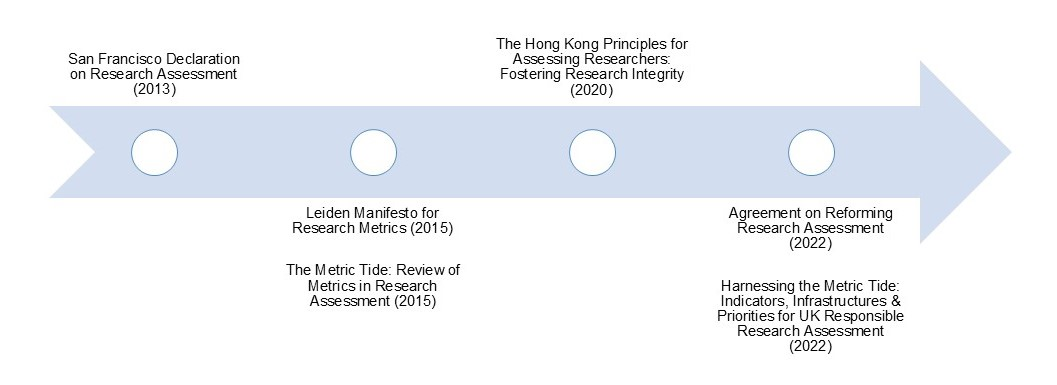
\includegraphics{images/figures/researchassessment-timeline.jpg}

}

\caption{\label{fig-milestones}Milestones in the history of research
assessment reform}

\end{figure}%

Although the \href{https://sfdora.org/read/}{San Francisco Declaration
on Research Assessment} (DORA, 2013), the founding text of research
assessment reform, was primarily concerned with research publications
and related metrics, its second recommendation adumbrates a broader
assessment agenda:

\begin{quote}
For the purposes of research assessment, consider the value and impact
of all research outputs (including datasets and software) in addition to
research publications, and consider a broad range of impact measures
including qualitative indicators of research impact, such as influence
on policy and practice.
\end{quote}

But while DORA mentions datasets and software as examples of other
research outputs, it lacks the broader concept of open research that has
developed in the years since its publication, and it does not provide
any guidance on how other types of output might be included and
assessed. The \href{https://doi.org/10.1038/520429a}{Leiden Manifesto}
and the
\href{https://www.ukri.org/publications/review-of-metrics-in-research-assessment-and-management/}{Metric
Tide report} (both published in 2015) were similarly focused on the use
of publication metrics.

More recently a broader framework of responsible research assessment has
emerged,\footnote{`The focus on responsible metrics has now been folded
  into the broader framework of responsible research assessment (RRA).
  This can be defined as ``an umbrella term for approaches to assessment
  which incentivise, reflect and reward the plural characteristics of
  high-quality research, in support of diverse and inclusive research
  cultures''.' Curry, S., Gadd, E. and Wilsdon J. (2022), `Harnessing
  the metric tide: indicators, infrastructures and priorities for
  responsible research assessment in the UK'. Research on Research
  Institute. \url{https://doi.org/10.6084/m9.figshare.21701624.v2},
  p.~23. The quotation refers to a paper from the Research on Research
  Institute that is perhaps the first to articulate this broader
  framework. See Curry, S. et al.~(2020). The changing role of funders
  in responsible research assessment: progress, obstacles and the way
  ahead (RoRI Working Paper No.3). 10.6084/m9.figshare.13227914.v2.
  Research on Research Institute.
  \url{https://doi.org/10.6084/m9.figshare.13227914.v2}} within which
increased attention to open research is evident. A white paper from the
League of European Universities (LERU) published in 2018 recommended
that universities `endeavour to integrate Open Science dimensions in
their HR and career frameworks as an explicit element in recruitment,
performance evaluation and career advancement policies'.\footnote{Ayris,
  P. et al (2018), `Open Science and its role in universities: a roadmap
  for cultural change'. League of European Research Universities.
  \url{https://www.leru.org/publications/open-science-and-its-role-in-universities-a-roadmap-for-cultural-change}.}
Also in 2018, the European Universities Association published the `EUA
Roadmap on Research Assessment in the Transition to Open Science', which
argued:

\begin{quote}
Today, research assessment and reward systems generally do not reflect
important Open Science contributions, such as curating and sharing
datasets and collections, documenting and sharing software (source
code), or devoting time and energy to high-quality peer review. New
approaches to research assessment that take into account Open Science
contributions need to be identified and thoroughly discussed by academic
communities.\footnote{European Universities Association (2018), `EUA
  Roadmap on Research Assessment in the Transition to Open Science'.
  \url{https://eua.eu/resources/publications/316:eua-roadmap-on-research-assessment-in-the-transition-to-open-science.html}.}
\end{quote}

The `Hong Kong Principles for assessing researchers' (2020) call for
assessment to develop a much broader picture of a researcher's
contributions to research and society. It identifies as one of its five
principles to `Reward the practice of open science (open research)', and
it makes a strong connection between research transparency and research
integrity.\footnote{Moher, D. et al.~(2020). `The Hong Kong Principles
  for assessing researchers: Fostering research integrity'. PLoS Biol
  18(7): e3000737. \url{https://doi.org/10.1371/journal.pbio.3000737}.}
The \href{https://doi.org/10.54677/MNMH8546}{UNESCO Recommendation on
Open Science} (2021) enjoined member states to remove barriers to open
science relating to research and career evaluation and awards systems,
stating: `Assessment of scientific contribution and career progression
rewarding good open science practices is needed for operationalization
of open science'.

In the
\href{https://coara.eu/agreement/the-agreement-full-text/}{Agreement on
Reforming Research Assessment}, published in 2022 by the Coalition for
Advancing Research Assessment (CoARA), `openness' is recognised as being
integral to the practices by which research is conducted, communicated
and validated, and is identified as a key dimension of research
assessment. Under the `Quality and impact' principle of research
assessment it states: `Openness of research, and results that are
verifiable and reproducible where applicable, strongly contribute to
quality'. Under the principle `Diversity, inclusiveness and
collaboration', signatories agree to:

\begin{quote}
Consider\ldots{} the full range of research outputs, such as scientific
publications, data, software, models, methods, theories, algorithms,
protocols, workflows, exhibitions, strategies, policy contributions,
etc., and reward research behaviour underpinning open science practices
such as early knowledge and data sharing as well as open collaboration
within science and collaboration with societal actors where appropriate.
\end{quote}

\section{National and institutional assessment practices need to
develop}\label{national-and-institutional-assessment-practices-need-to-develop}

The greater emphasis on open research in the research assessment reform
agenda is relatively recent, and national and institutional research
assessment policies have so far reflected a prevailing focus on
publications and the responsible use of publication metrics. In a survey
undertaken by the OR4 project in 2023, 44 or 73\% of 60 institutions
stated that they had a responsible research assessment statement or
policy. The majority of these were focused on the responsible use of
publication metrics.\footnote{Barnett, J. at al.~(2024). `OR4 Research
  Assessment Survey Report'. Working Paper No 5.
  \url{https://doi.org/10.31219/osf.io/z52cn}.} In scope and terminology
many of these statements follow and reference DORA and the Leiden
Manifesto.

The almost exclusive focus on the assessment of research publications is
understandable, given their prominence in the systems of academic
recognition and reward. In REF 2021, of 185,353 outputs submitted,
180,509 or 97.4\% fell into the main academic publications categories
A-E (including authored and edited books, book chapters, journal
articles and conference contributions). 154,826 outputs or 83.5\% of the
total were journal articles. The number of research data sets and
databases submitted was 31; the number of software outputs was 11
(Figure~\ref{fig-refoutputs}).\footnote{REF 2021 Submitted outputs'
  details. \url{https://results2021.ref.ac.uk/outputs}.}

\begin{figure}

\centering{

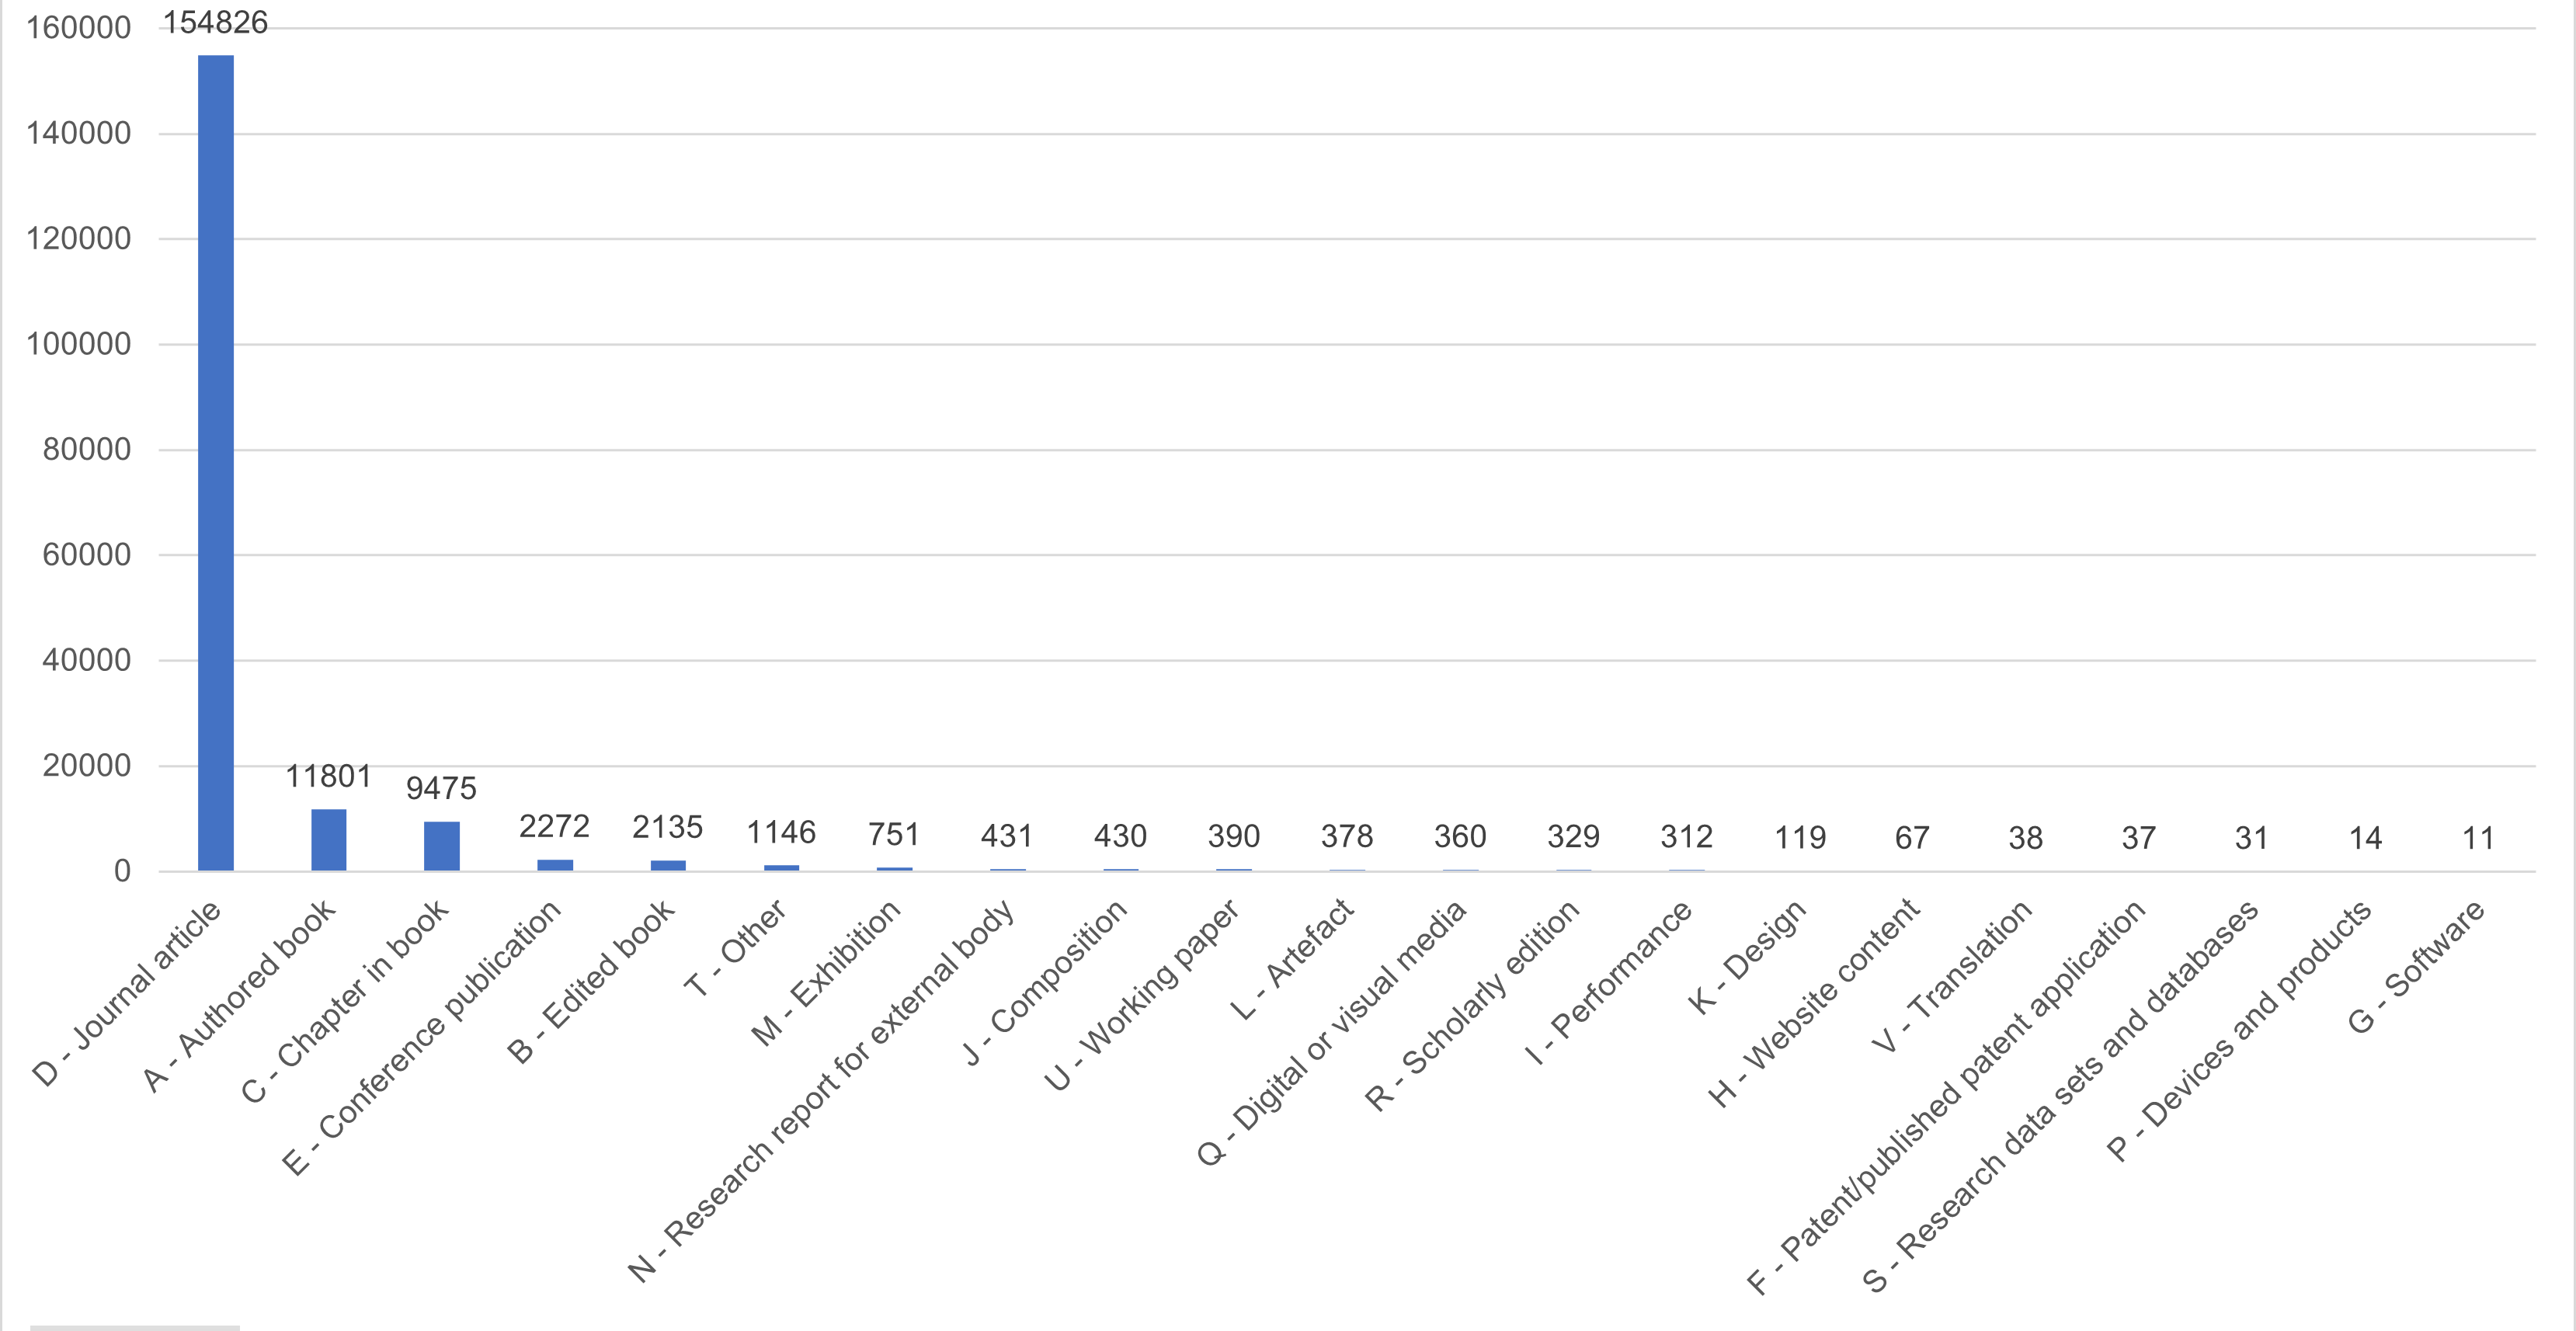
\includegraphics{images/figures/ref-outputs.png}

}

\caption{\label{fig-refoutputs}REF 2021 submitted outputs by output
type}

\end{figure}%

This heavily skewed distribution is the focus of the
\href{https://hidden-ref.org/}{Hidden REF} initiative, which emerged in
the runup to the 2021 REF. This campaign highlighted the lack of
representation in submissions for non-academic research contributors
(such as data scientists, technicians and research software engineers)
and for `non-traditional' outputs (i.e.~other than publications). Now
that the UK is on track for REF 2029, the Hidden REF is campaigning on a
\href{https://hidden-ref.org/the-5-percent-manifesto/}{5\% manifesto}: a
target for HEIs to submit at least 5\% of non-traditional research
outputs. This will be a challenging target to meet, given that in REF
2021 only 2.4\% of non-traditional outputs were submitted.

But the landscape is beginning to change, and institutions will need to
develop policies that better align to the principles of responsible
research assessment and that are more representative of the full
diversity of research and research-related activities and outputs.

\section{The changing national and international research assessment
environment}\label{the-changing-national-and-international-research-assessment-environment}

In comparison to previous national assessment exercises, REF 2029 places
greater emphasis on institutional research culture, including use of
open research practices. Institutions can provide evidence of this in
the People, Culture and Environment element, while the element
Contribution to Knowledge and Understanding enables a greater diversity
of research activities and outputs to be evidenced.\footnote{Research
  England (2023), `Research Excellence Framework 2028: Initial decisions
  and issues for further consultation'.
  \url{https://www.ukri.org/publications/ref2028-initial-decisions-and-issues-for-further-consultation/}.}

As the national research assessment framework progressively assimilates
open research objectives and assessment criteria, institutions will be
obliged to conform, and to integrate open research into their own
policies, systems and processes. The greater emphasis on open research
in the 2029 REF is consistent with international developments, where
other national research environments are also beginning to demonstrate
greater alignment to the principles embodied in the Agreement on
Reforming Research Assessment, and to identify open research as an
important element of incentive and reward systems.

\begin{tcolorbox}[enhanced jigsaw, titlerule=0mm, coltitle=black, toprule=.15mm, title=\textcolor{quarto-callout-note-color}{\faInfo}\hspace{0.5em}{Open research in other national research assessment frameworks}, colframe=quarto-callout-note-color-frame, bottomrule=.15mm, opacityback=0, leftrule=.75mm, rightrule=.15mm, arc=.35mm, toptitle=1mm, colbacktitle=quarto-callout-note-color!10!white, opacitybacktitle=0.6, bottomtitle=1mm, breakable, left=2mm, colback=white]

\begin{itemize}
\item
  In the Netherlands, a 2020 report by the National Programme on Open
  Science argued that reform was needed on three levels: at the level of
  national assessment, at the institutional level, and at the level of
  funding agencies. The roadmap for the Dutch Recognition and Rewards
  Programme identifies open science as a priority, and aims to `clarify
  how activities relating to open science and open education will be
  considered and/or prioritised as a topic of discussion in the
  development, assessment, appointment and promotion of
  staff'.\footnotemark{}
  \href{https://www.nwo.nl/en/researchprogrammes/open-science/open-science-fund}{Funding}
  has since been ringfenced by the Dutch Research Council (NWO) to
  support implementation and stimulation of open science culture and
  practices.
\item
  In 2021 Universities Norway published
  \href{https://www.uhr.no/en/news-from-uhr/nor-cam-a-toolbox-for-recognition-and-rewards-in-academic-careers.5780.aspx}{NOR-CAM},
  a national research assessment framework that integrates open science
  principles in the assessment of academic results, activities and
  competencies. NOR-CAM was developed from the Open Science Career
  Assessment Matrix (OS-CAM).\footnotemark{}
\item
  The Irish National Action Plan for Open Research published in 2022
  calls for an alignment of research assessment with the principles of
  open research at both national and institutional level as part of
  action to establish a culture of open research, and proposes among
  other actions Adoption of a modified OS-CAM model to the national
  context.\footnotemark{}\\
\end{itemize}

\end{tcolorbox}

\footnotetext{Hans de Jonge (2023), `Open science and recognition \&
rewards: what's the link between them?' Recognition \& Rewards: Embrace
the Impact.
\url{https://recognitionrewardsmagazine.nl/2023/open-science/}.}

\footnotetext{Working Group on Rewards under Open Science (2017),
`Evaluation of research careers fully acknowledging Open Science
practices'. \url{https://data.europa.eu/doi/10.2777/75255}.}

\footnotetext{NORF (2022). National Action Plan for Open Research.
\url{https://doi.org/10.7486/DRI.ff36jz222}.}

\section{Challenges of including open research in institutional
research(er)
assessment}\label{challenges-of-including-open-research-in-institutional-researcher-assessment}

Ensuring the meaningful inclusion of open research objectives in
institutional researcher assessment and aligned research planning
activities at all levels in an institution is a long-term challenge
requiring a sustained effort of leadership and co-ordinated activity.
Challenges can be summarised as political, cultural, practical and
operational.

\subsection{Political}\label{political}

There is substantial institutional investment in the prevailing
publication-based model of research assessment. Institutional research
KPIs and research elements of league table rankings are largely defined
by publication metrics. Not all research leaders, managers, and
researchers will agree that use of open research practices is a relevant
criterion of research assessment, and securing buy-in to support policy
adoption and implementation across relevant procedures may not be
straightforward.

\subsection{Cultural}\label{cultural}

There will be similar challenges securing engagement and bringing about
changes in practice among members of the research community at large, in
their capacity as both assessors and subjects of research assessment.
Many will not have fully integrated open research practices into their
working methods and may have concerns they would be disadvantaged. Care
will need to be taken that where open research criteria are introduced
in assessment practices their use is fair and equitable. Ability to
evidence open research practice will depend on the discipline and type
of research, and the background and career stage of a researcher.
Researchers may have lacked the training, means or opportunity to use
open research practices. All of these factors will necessitate the
provision of guidance, training and support in the context of sustained
activity to develop and enable a culture of open research practice.

\subsection{Practical}\label{practical}

The institution will need an effective operating definition of open
research. Researchers and those involved in the assessment of
researchers will need to be equipped to identify activities and outputs
that fall under that definition, to make an assessment of the degree to
which an activity or output fulfils qualifying criteria, and to appraise
the value of the activity or output within the context of the assessment
as a whole. Each of these requirements presents its own challenges. Many
academics may struggle to identify open outputs, or fail to appreciate
the difference between, say, a dataset that is published on a project
website without a licence and one that has been deposited in a data
repository under an open licence and assigned a DOI.

It is also the case that for many open research outputs there is no
pre-publication peer review, and standards of assessment may be
difficult to define and apply across a variety of outputs, even of the
same type, meaning that outputs often lack markers of certification. It
is also often difficult to obtain reliable, comparable quantitative
information about the citation and use of many open research outputs.

\subsection{Operational}\label{operational}

There will be the complex work of implementing changes to policies and
procedures, and underpinning systems, processes and support, creating
and delivering guidance and training, monitoring compliance with
implemented policies and taking follow-up action as required. This may
entail development of or addition to existing systems and processes.
Systems for management and assessment of research are based in large
part on research publications, which are well-defined entities that
support citation, quantification and comparison. Mature infrastructure,
systems and processes facilitate their dissemination, and the collection
and processing of information about them. Models for the integration of
open research into institutional research assessment and research
planning are yet to be established; but if research assessment is to
accommodate a wider range of activities and outputs, this will introduce
complexity and additional operational demand.

The OR4 implementation guide addresses these aspects of implementation,
with an emphasis on the political and cultural aspects in the earlier
sections moving into the practical and operational aspects in the later
sections.

\bookmarksetup{startatroot}

\chapter{Institutional commitment}\label{institutional-commitment}

\begin{tcolorbox}[enhanced jigsaw, colback=white, toprule=.15mm, colframe=quarto-callout-color-frame, arc=.35mm, opacityback=0, bottomrule=.15mm, breakable, left=2mm, leftrule=.75mm, rightrule=.15mm]

Does your institution make public commitments to the principles and aims
of open research and responsible research assessment, which are aligned
to the direction of travel in the sector and supported by effective
action?

\end{tcolorbox}

\section{Why is this important?}\label{why-is-this-important}

\begin{itemize}
\item
  Expressions of institutional commitment can send a strong message that
  open research and responsible research assessment are matters of
  strategic importance to the institution and its leadership.
\item
  The process of consulting on and formulating a statement of commitment
  can engage key stakeholders and create a shared sense of purpose and
  strategic direction, providing a foundation for effective action.
\item
  The institution can ensure that recognition and reward for open
  research is within the scope of research assessment reform and that
  where strategic action on open research and research assessment reform
  are separately undertaken, activity leads/groups are agreed on common
  objectives and co-ordinated in their activities.
\item
  Public alignment to influential statements such as the UNESCO
  Recommendation on Open Science, DORA and CoARA signals that the
  necessity for cultural change is widely accepted in the sector and
  that the institution and its members must adapt. Membership of CoARA
  provides access to working groups that can support sharing of good
  practice and implementation.
\end{itemize}

\section{Maturity scale}\label{maturity-scale}

\begin{longtable}[]{@{}
  >{\raggedright\arraybackslash}p{(\columnwidth - 6\tabcolsep) * \real{0.2500}}
  >{\raggedright\arraybackslash}p{(\columnwidth - 6\tabcolsep) * \real{0.2500}}
  >{\raggedright\arraybackslash}p{(\columnwidth - 6\tabcolsep) * \real{0.2500}}
  >{\raggedright\arraybackslash}p{(\columnwidth - 6\tabcolsep) * \real{0.2500}}@{}}
\toprule\noalign{}
\begin{minipage}[b]{\linewidth}\raggedright
No Action
\end{minipage} & \begin{minipage}[b]{\linewidth}\raggedright
Emerging
\end{minipage} & \begin{minipage}[b]{\linewidth}\raggedright
Evolving
\end{minipage} & \begin{minipage}[b]{\linewidth}\raggedright
Sustained
\end{minipage} \\
\midrule\noalign{}
\endhead
\bottomrule\noalign{}
\endlastfoot
There are no public institutional commitments to open research and
responsible research assessment. & There are public institutional
commitments to open research and responsible research assessment but
little or no recognition of open research in research assessment
practice. & There are public institutional commitments to open research
and responsible research assessment. There is an explicit commitment to
recognise and reward open research in research assessment practice. &
Public open research and responsible research assessment commitments are
well-integrated into recognition and reward policies and procedures.
There is a strong shared understanding of how open research and
responsible research assessment contribute to institutional research
strategy and overall mission. \\
\end{longtable}

\section{Progress actions}\label{progress-actions}

Here are suggestions for key actions that can be taken to progress from
one level of the maturity framework to the next. These can be considered
when you develop an institutional action plan.

\subsection{No Action to Emerging}\label{no-action-to-emerging}

\begin{itemize}
\item
  Adopt and publish an open research statement.
\item
  Adopt and publish a commitment to the implementation of responsible
  research assessment. This could be held within the wider open research
  statement.
\item
  Sign the Agreement on Reforming Research Assessment and join the
  Coalition on Advancing Research Assessment (CoARA) and communicate
  this within the institution.
\end{itemize}

\subsection{Emerging to Evolving}\label{emerging-to-evolving}

\begin{itemize}
\item
  Initiate action to implement commitments, e.g.~by appointment of
  senior strategic leads for open research and responsible research
  assessment, development and publication of action plans, and
  engagement of key stakeholders.
\item
  Include a commitment to recognise and reward open research practice
  within institutional research assessment.
\item
  Ensure senior leads and stakeholder groups (where they have been
  established) are co-ordinated towards objectives for recognition and
  reward for open research.
\item
  Demonstrate that progress has been made in implementing commitments,
  e.g.~by publishing updates against action plan milestones.
\end{itemize}

\subsection{Evolving to Sustained}\label{evolving-to-sustained}

\begin{itemize}
\item
  Ensure that commitments are well-integrated into relevant policies,
  procedures, assessment, guidance and training, and that they are
  widely understood and supported by research leaders and managers.
\item
  Ensure that activities and communications relating to institutional
  research strategy, environment and culture are aligned to and
  reference institutional commitments.
\end{itemize}

\section{Main areas of activity}\label{main-areas-of-activity}

\subsection{Open research statement}\label{open-research-statement}

Increasing numbers of UK universities, and indeed institutions globally,
are adopting public institutional statements of commitment to the
principles and aims of open research.\footnote{Sheppard, N. (2020, since
  updated), `Open access is not enough: reproducible science, research
  and scholarship'. UKCORR. Blogpost.
  \url{https://www.ukcorr.org/2020/12/02/open-access-is-not-enough-reproducible-science-research-and-scholarship/}.}
Their function is to provide the strategic commitment to develop a
culture of open research and the high-level framework under which
activity and policies (such as those on open access and data sharing)
can sit. The statement should be in alignment with (and may reference)
the University's research strategy.

It is preferable for the statement to include a commitment to recognise
and reward open research practice within institutional assessment. It
should reference an institutional statement or policy on responsible
research assessment this exists. Reference to statements such as the
\href{https://www.ukri.org/what-we-do/supporting-healthy-research-and-innovation-culture/open-research/}{UKRI
position on open research} and the
\href{https://www.unesco.org/en/open-science/about?hub=686}{UNESCO
Recommendation on Open Science} can serve to emphasise alignment to the
sector.

Members of the institution formulating this commitment will need to
reflect on how open research is understood within the context of the
institutional mission, and how it contributes to the advancement of that
mission.

\subsection{Research assessment
reform}\label{research-assessment-reform}

With momentum for research assessment reform building globally, many
institutions are reviewing or planning to review their research
assessment policies and procedures. This may entail publishing or
refreshing a statement of commitment to the agenda of research
assessment reform.

Many institutions have already signed the
\href{https://sfdora.org/read/}{San Francisco Declaration on Research
Assessment} (DORA) and will have made a commitment to improve research
and researcher assessment within their institutions. As of 7th November
2022, DORA asked signatory institutions to `share a public statement
detailing their commitment to DORA and responsible research assessment
to their communities'.\footnote{DORA (2022), `Engagement and outreach
  policy'. \url{https://sfdora.org/sign/}.}

Whether or not institutions are DORA signatories, there is a case for
signing the Agreement on Reforming Assessment to begin the process of
establishing specific commitments and a timetable of reform. Signatories
commit to develop and share with CoARA within one year of signing the
Agreement an \href{https://coara.eu/agreement/action-plan/}{action plan}
for reviewing or developing criteria, tools and processes in line with
the core Commitments. They also agree to regularly demonstrate progress
against this action plan, with a touch point within five years of
signing the Agreement.

Institutions that receive funding from the
\href{https://wellcome.org/grant-funding/guidance/open-access-guidance/research-organisations-how-implement-responsible-and-fair-approaches-research}{Wellcome
Trust} are also required to publish on their website a commitment to the
use of responsible research assessment aligned with the DORA and CoARA
principles. They are expected to have a plan in place for implementing
the principles, and for monitoring and reporting on implementation.

A statement of institutional commitment to research assessment reform
should include an undertaking to integrate open research criteria into
systems of reward and recognition, in line with the emphasis placed on
open research/open science in the Agreement and
\href{guide-intro.qmd}{more recent discussions of responsible research
assessment}. It should also reference the statement of institutional
commitment to open research, where this exists.

\subsection{Supporting commitments}\label{supporting-commitments}

Aside from commitment explicitly based on or subscribing to the main
research assessment reform initiatives, institutions might consider
making supporting commitments, e.g.:

\begin{itemize}
\item
  The \href{https://inorms.net/more-than-our-rank/}{More than Our Rank}
  initiative provides an opportunity for academic institutions to
  highlight the problematic nature of league table rankings.
\item
  the Hidden REF 5 \% Manifesto encourages institutions to commit to
  submit at least 5\% of their submissions to REF 2029 as
  non-traditional research outputs, to promote better representation for
  the range of research contribution roles and `non-traditional'
  research outputs.
\end{itemize}

Whether or not institutions sign up to all these commitments, discussion
of them can be useful ways to highlight areas of practice in need of
reform and to consider ways in which they might be addressed.

\subsection{Building commitment}\label{building-commitment}

Publishing commitments to open research or research assessment reform
will be a collective effort, with stakeholder groups led by senior
colleagues. Any commitment will be ineffective if the effort is not made
to build the coalition that will implement it and if ownership and
accountability are not built in. The process of developing an
institutional statement will offer an opportunity to engage stakeholders
through consultation, to secure support for their achievement through
strategic actions. Care should be taken to ensure that relevant
stakeholder groups are represented in the process of developing and
consulting on institutional commitments (including, for example, early
career researchers and professional services colleagues) and that
statements, once adopted, are communicated to the research community.
Institutional commitments will need to be signed off at a high level,
and there will need to be appropriate ownership of, and accountability
for, delivering against the commitments.

Strategic activities related to development of open research and
research assessment reform may have separate origins within the
institution and may be undertaken by separate groups under different
leadership. Where this is the case, it will be important to ensure that
their activities are co-ordinated on the common ground of reward and
recognition for open research, and that there is agreement about
objectives and the means of attainment. The process of developing and
consulting on institutional statements should ensure this co-ordination
and agreement take place.

Agreement on the relevance and place of open research within research
assessment cannot be taken for granted. One advantage of signing up to
the Agreement on Reforming Research Assessment is that by doing so the
institution subscribes to the Core Commitment to `Recognise the
diversity of contributions to, and careers, in research in accordance
with the needs and nature of the research'. The purpose of this
Commitment is to broaden the range of research activities and outputs
recognised, to include inter alia `diverse outputs beyond journal
publications' and `practices that contribute to robustness, openness,
transparency and the inclusiveness of research'.

\subsection{Demonstrating progress in implementing the
commitments}\label{demonstrating-progress-in-implementing-the-commitments}

The institution will need to demonstrate over time that aspirational
commitments are being realised and incorporated into business as usual.
Published commitments can identify senior leads and groups responsible
for implementing them, and include action plans and updates on progress
against milestones. Where there are specific reporting expectations
associated with external commitments, such as those associated with
membership of \href{https://coara.eu/agreement/action-plan/}{CoARA},
these can be communicated within the institution.

Activities and communications relating to institutional research
strategy, environment and culture should be aligned to and reference
institutional commitments. Policies and procedures will in due course
integrate elements of the open research commitments that have been
realised and may reference them, as may relevant guidance and training.
Internal communication channels can be used to communicate the open
research commitments to key stakeholders and the broader research
community. Management structures can be used to ensure the commitments
are applied and referenced as appropriate.

\bookmarksetup{startatroot}

\chapter{Leadership}\label{leadership}

\begin{tcolorbox}[enhanced jigsaw, colback=white, toprule=.15mm, colframe=quarto-callout-color-frame, arc=.35mm, opacityback=0, bottomrule=.15mm, breakable, left=2mm, leftrule=.75mm, rightrule=.15mm]

Does your institution provide leadership at a senior level for strategic
action on open research and responsible research assessment, including
recognition and reward for open research, and is open research
leadership fostered at all levels in the institution?

\end{tcolorbox}

\section{Why is this important?}\label{why-is-this-important-1}

\begin{itemize}
\item
  Recognition and reward for open research may be implemented at the
  intersection of strategic activities to develop open research culture
  and to undertake research assessment reform. Where these activities
  are separately led, leaders in both areas must accept and agree on the
  objectives to be achieved, in order for implementation to be
  effective.
\item
  Recognition and reward for open research in research assessment is
  relatively undeveloped. There is a risk that the importance of
  recognising and rewarding open research will not be appreciated or
  factored into activity. It will be essential to have an informed and
  empowered advocate who is able to ensure open research is within scope
  of activity and given due weight.
\item
  Leadership can be demonstrated by those in positions of influence, as
  research leaders and managers and senior members of professional
  services, as colleagues who might support good practice though the
  provision of services, guidance and training e.g., organisational
  culture or HR representatives, and as informal or nominated advocates
  of open research.
\end{itemize}

\section{Maturity scale}\label{maturity-scale-1}

\begin{longtable}[]{@{}
  >{\raggedright\arraybackslash}p{(\columnwidth - 6\tabcolsep) * \real{0.2500}}
  >{\raggedright\arraybackslash}p{(\columnwidth - 6\tabcolsep) * \real{0.2500}}
  >{\raggedright\arraybackslash}p{(\columnwidth - 6\tabcolsep) * \real{0.2500}}
  >{\raggedright\arraybackslash}p{(\columnwidth - 6\tabcolsep) * \real{0.2500}}@{}}
\toprule\noalign{}
\begin{minipage}[b]{\linewidth}\raggedright
No Action
\end{minipage} & \begin{minipage}[b]{\linewidth}\raggedright
Emerging
\end{minipage} & \begin{minipage}[b]{\linewidth}\raggedright
Evolving
\end{minipage} & \begin{minipage}[b]{\linewidth}\raggedright
Sustained
\end{minipage} \\
\midrule\noalign{}
\endhead
\bottomrule\noalign{}
\endlastfoot
There is no senior strategic leadership for open research or responsible
research assessment. & There are identified senior strategic leads for
open research and responsible research assessment. Recognition and
reward for open research in research assessment is an identified
priority for strategic action. & Senior leadership develops actions on
open research and responsible research assessment in collaboration with
key stakeholders. Actions to recognise open research in research
assessment are agreed and supported by relevant leads and promoted by
open research advocates across the institution. & Recognition and reward
for open research in research assessment is progressed as a strategic
priority by members of senior management. External engagement ensures
alignment to sector. Leadership in open research is seen and valued
across the organisation, and includes researchers, research enablers and
open research advocates. \\
\end{longtable}

\section{Progress actions}\label{progress-actions-1}

Here are suggestions for key actions that can be taken to progress from
one level of the maturity framework to the next. These can be considered
when you develop an institutional action plan.

\subsection{No Action to Emerging}\label{no-action-to-emerging-1}

\begin{itemize}
\item
  Nominate and empower a member of senior management or professional
  services with responsibility for strategic action to develop open
  research culture and practice.
\item
  Nominate and empower a senior strategic lead for responsible research
  assessment.
\item
  Identify recognition and reward for open research as a priority for
  strategic action.
\end{itemize}

\section{Emerging to Evolving}\label{emerging-to-evolving-1}

\begin{itemize}
\item
  Evidence sustained activity by senior strategic leads for open
  research and responsible research assessment and engagement with
  relevant stakeholders. Where leadership of open research and
  responsible research assessment is separate, ensure there is
  co-ordinated actions and agreement on objectives to include
  recognition and reward for open research.
\item
  Identify and develop advocates in the research community and
  professional services who can provide leadership and support for open
  research recognition and reward.
\end{itemize}

\section{Evolving to Sustained}\label{evolving-to-sustained-1}

\begin{itemize}
\item
  Demonstrate progress in embedding culture change under the direction
  of the senior strategic lead.
\item
  Cascade open research leadership through the organisation, with
  research leaders and managers, research professionals and other
  champions showing leadership in open research in their areas of
  activity and influence.
\item
  Demonstrate that championing open research practice is a recognised
  criterion of research leadership, for example through inclusion in job
  descriptions, promotion criteria, annual performance and development
  review.
\item
  Demonstrate that leadership in the institution is engaging externally
  with research assessment reform networks in order to promote effective
  recognition and reward for open research at a national level.
\end{itemize}

\section{Main areas of activity}\label{main-areas-of-activity-1}

\subsection{Open research leadership}\label{open-research-leadership}

A member of senior management with responsibility for developing open
research culture and practice within the institution can develop and
lead strategic action and act as a senior champion for open research.
This person will represent the institutional commitment to open research
and act as a strong advocate for the open research interest. They must
be sufficiently informed about open research and convinced of its
importance to be a strong advocate. This will be essential where
research assessment reform activity is separately led, and discussion
may be required to ensure that recognition and reward for open research
is within scope of activity and given appropriate weight.

An open research lead is likely to have greatest impact when this is a
role with authority to instigate institution-wide change e.g., a dean,
senior professional services manager, or someone at a similar level. It
is preferable for the role to have some FTE commitment with defined
responsibilities and accountability, for example to develop, implement
and report on the progress of a plan of strategic action to increase
open research culture and practice in the institution. For members of
the UKRN, the role could fit well with that of Institutional Lead:
members of the UKRN are required to appoint a senior academic to this
role, with responsibility for research improvement and research
integrity, reporting to the PVC for Research (or their equivalent). The
Institutional Lead role is expected to make a minimum commitment of 1
day per week (0.2FTE). Stakeholders within institutions that lack an
open research lead and are not currently members of UKRN may be able to
use the case for membership as a vehicle for securing senior management
leadership for open research.

Action to develop open research culture and practice in the institution
would ideally be undertaken by a group convened for the purpose under
the senior lead for open research and comprising representatives of key
stakeholder groups, including representatives of the academic community
and relevant professional services. However, the scope of this group,
and its actions, are anticipated to vary across institutions based upon
research priorities and available resources.

\subsection{Leadership in recognition and reward for open
research}\label{leadership-in-recognition-and-reward-for-open-research}

Implementation of recognition and reward for open research will require
leadership in promoting the need for change within the institution,
engaging key stakeholders and the wider community to secure buy-in and
manage resistance, and in managing a stakeholder group tasked with
delivering established objectives.

Implementation may sit at the intersection of otherwise separate
activities to address research assessment reform and to develop open
research culture and practice. These activities may be undertaken by
separate groups under the direction of different senior leads within the
institution. Where this is the situation, the lead for open research
will need to make the case for recognition of open research within
institutional assessment and ensure that there is agreement with the
lead for research assessment reform on the objectives to be achieved and
the means by which they will be achieved. This agreement may have been
established through the process of developing institutional commitments
to open research and research assessment reform.

\subsection{External engagement}\label{external-engagement}

While the focus of senior leadership roles will be on activity within
the institution, there will also be opportunities for external
engagement. Leadership here may help to promote alignment in policies
for recognition of open research within research assessment, at the
level of national assessment (i.e.~through the REF), by funders when
assessing researchers and institutions for the award of grants, and
between institutions, so that researchers are assessed by similar
standards at all institutions. Representation in national fora such as
the
\href{https://coara.eu/coalition/national-chapters/coara-national-chapter-uk-2/}{CoARA
National Chapter} (for CoARA members) and the OR4 Community of Practice
afford opportunities to exchange knowledge and practice and to
co-ordinate activities across the UK sector.

\subsection{Research leaders and
managers}\label{research-leaders-and-managers}

Research leaders and managers have a role to play in developing a
research environment that incentivises researchers to use open research
practices, as well as in the specific promotion of recognition and
reward for open research. According to their roles and institutional
requirements they may do any of the following:

\begin{itemize}
\item
  promote the use of open research practices in the areas under their
  authority, including relevant policy expectations, such as those
  relating to open access publication and data sharing;
\item
  set an example by demonstrating good open research practice in their
  own work and professional relationships;
\item
  use communication activities to highlight and celebrate the open
  research activities and outputs of colleagues;
\item
  engage with and signpost to colleagues the professional services that
  provide support for open research, such as research publishing and
  research data management services;
\item
  support researchers at all levels to develop their knowledge and
  skills through the training and support provided by the institution;
\item
  use research planning and internal review processes to identify and if
  required report on attainment of open research objectives at group or
  individual level, as relevant;
\item
  monitor activity and compliance, and take appropriate action in cases
  of non-compliance or poor practice, such as arranging for additional
  support or training;
\item
  ensure that activities involving the assessment of researchers under
  their authority (e.g.~recruitment and probation, promotion,
  performance and development review, etc.) implement appropriate
  recognition and reward for open research.
\end{itemize}

\subsection{Other leadership roles}\label{other-leadership-roles}

Leadership will also be required at different levels and in different
places in the institution to champion the open research agenda, and
specific activity to include recognition and reward for open research in
research assessment. Champions may be:

\begin{itemize}
\item
  Members of professional services who will support implementation: both
  those who provide open research support and training and have a strong
  investment in promoting open research practice, and others such as HR
  professionals who may have specific roles to play in implementing and
  promoting new policies and procedures;
\item
  Advocates for good practice in research, who may be formally nominated
  in some capacity, or have some informal role. Examples include open
  research champions, UK Reproducibility Network Local Network Leads,
  etc.
\end{itemize}

\bookmarksetup{startatroot}

\chapter{Strategy and planning}\label{strategy-and-planning}

\begin{tcolorbox}[enhanced jigsaw, colback=white, toprule=.15mm, colframe=quarto-callout-color-frame, arc=.35mm, opacityback=0, bottomrule=.15mm, breakable, left=2mm, leftrule=.75mm, rightrule=.15mm]

Do you have a strategic plan owned by a stakeholder group for developing
open research culture and practice, and is recognition and reward for
open research addressed in this plan and any related policies/plans
concerning the assessment of researchers?

\end{tcolorbox}

\section{Why is this important?}\label{why-is-this-important-2}

\begin{itemize}
\item
  Recognition and reward for open research practice must be situated
  within wider strategic activity to develop open research culture and
  practice in the institution. Researchers could lack awareness of open
  research or the motivations, skills and resources to effectively adopt
  open research practices.
\item
  Implementing recognition and reward for open research should be a key
  element of research assessment reform.
\item
  Implementing expectations related to open research in research
  assessment will not be effective if the institution does not also
  develop policy and infrastructure, and provide information, training
  and support to create an environment in which open research practice
  is enabled and incentivised.
\end{itemize}

\section{Maturity scale}\label{maturity-scale-2}

\begin{longtable}[]{@{}
  >{\raggedright\arraybackslash}p{(\columnwidth - 6\tabcolsep) * \real{0.2500}}
  >{\raggedright\arraybackslash}p{(\columnwidth - 6\tabcolsep) * \real{0.2500}}
  >{\raggedright\arraybackslash}p{(\columnwidth - 6\tabcolsep) * \real{0.2500}}
  >{\raggedright\arraybackslash}p{(\columnwidth - 6\tabcolsep) * \real{0.2500}}@{}}
\toprule\noalign{}
\begin{minipage}[b]{\linewidth}\raggedright
No Action
\end{minipage} & \begin{minipage}[b]{\linewidth}\raggedright
Emerging
\end{minipage} & \begin{minipage}[b]{\linewidth}\raggedright
Evolving
\end{minipage} & \begin{minipage}[b]{\linewidth}\raggedright
Sustained
\end{minipage} \\
\midrule\noalign{}
\endhead
\bottomrule\noalign{}
\endlastfoot
There is no open research strategy or plans to implement change. & A
strategic plan for open research has identified recognition and reward
for open research in research assessment as an area for action. This
objective is recognised in strategic action on research assessment
reform. & Strategic action on open research has progressed. Recognition
and reward for open research across all key areas of research assessment
is actioned by a stakeholder group against a strategic plan. Progress
has been made against objectives. & Strategic action on open research is
well-developed and sustained. Recognition and reward for open research
has been implemented in relevant policies and procedures. The
implementation plan has been delivered and action is focused on
monitoring, consolidating and embedding practice. \\
\end{longtable}

\section{Progress actions}\label{progress-actions-2}

Here are suggestions for key actions that can be taken to progress from
one level of the maturity framework to the next. These can be considered
when you develop an institutional action plan.

\subsection{No Action to Emerging}\label{no-action-to-emerging-2}

\begin{itemize}
\item
  Create and secure approval for a strategic action plan to develop open
  research culture and practice which identifies recognition and reward
  for open research as an area for action.
\item
  Where research assessment reform work is undertaken by an existing
  group, ensure that there is representation for open research in this
  group.
\item
  Establish recognition and reward for open research as an objective,
  and discuss the infrastructure, training, and support that may be
  required.
\end{itemize}

\subsection{Emerging to Evolving}\label{emerging-to-evolving-2}

\begin{itemize}
\item
  Demonstrate progress against an open research action plan.
\item
  Ensure there is a group, sub-group and/or detailed plan for
  implementing research assessment reform, including recognition and
  reward for open research, which is agreed and owned by the relevant
  stakeholder group.
\item
  Demonstrate progress against the research assessment reform
  implementation plan, with members of the stakeholder group working to
  deliver primary objectives.
\end{itemize}

\subsection{Evolving to Sustained}\label{evolving-to-sustained-2}

\begin{itemize}
\item
  Demonstrate that substantive progress has been made against the action
  plan to develop open research culture and practice.
\item
  Demonstrate that primary objectives of the research assessment reform
  implementation plan have been delivered, with recognition and reward
  for open research integrated into all relevant research assessment
  policies and procedures.
\item
  Move from implementation to a consolidation and embedding of
  operational activity, with monitoring and reporting to the relevant
  oversight committee/group.
\end{itemize}

\section{Main areas of activity}\label{main-areas-of-activity-2}

\subsection{Open research action plan}\label{open-research-action-plan}

A strategic action plan to develop open research culture and practice
may be created and implemented. The plan is likely to identify
objectives, deliverables, dates, responsibilities and measures of
attainment, and needs to be supported by a commitment of staff time and
other resources required for effective implementation. The plan needs to
be managed on an ongoing basis, and to demonstrate and report progress
against specified milestones to a relevant committee with
oversight.\footnote{UKRN provides a `Checklist for an Open Research
  Action Plan': \url{https://www.ukrn.org/primers/}. Examples of plans
  developed by different institutions include: Keele,
  \url{https://tinyurl.com/2wehf9xr}; Reading,
  \url{https://tinyurl.com/murfjnf2}; Surrey,
  \url{https://tinyurl.com/5n7mtbe2}.} It should include as one of its
objectives to implement recognition and reward for open research in
institutional assessment systems.

Implementation of recognition and reward for open research may not be
directly owned by an open research stakeholder group, as it is likely to
sit within wider activity on assessment or similar. An open research
lead should ensure that relevant research assessment reform objectives
are within the scope of the activity and are appropriately defined and
owned by this group. In practice this should entail someone on groups
responsible for assessment having a specific brief to represent the open
research interest.

Recognition and reward for open research will be one primary objective
of the open research strategic plan, which will be enabled by more
general progress in developing the culture and practice of open research
in the institution. As open research is progressively established in the
mainstream of institutional research activities, and as open research
practice increases, it will become more usual for researchers to
evidence the use of open research practices when presenting their work,
and for this to be expected and recognised by those involved in the
assessment of researchers.

\subsection{Implementing recognition and reward for open research in
research assessment
reform}\label{implementing-recognition-and-reward-for-open-research-in-research-assessment-reform}

Within plans for research assessment reform, recognition and reward for
open research should be included. This is likely to affect many areas of
assessment activity, including the development of policy and procedures,
and any guidance, training and support. Open research expertise will be
necessary to ensure open research is fully integrated into all aspects
of the implementation plan and that these elements are delivered as work
progresses.

Recognition and reward for open research can be addressed as part of
planning to meet the first Core Commitment, to `Recognise the diversity
of contributions to, and careers, in research in accordance with the
needs and nature of the research'. The purpose of this Commitment is to
broaden the range of research activities and outputs recognised, to
include inter alia `diverse outputs beyond journal publications' and
`practices that contribute to robustness, openness, transparency and the
inclusiveness of research'. This Commitment can be linked to the
`Diversity, inclusiveness and collaboration' Principle, which discusses
a wide range of research outputs and explicitly mentions open science
practices.

\bookmarksetup{startatroot}

\chapter{Communication and
engagement}\label{communication-and-engagement}

\begin{tcolorbox}[enhanced jigsaw, colback=white, toprule=.15mm, colframe=quarto-callout-color-frame, arc=.35mm, opacityback=0, bottomrule=.15mm, breakable, left=2mm, leftrule=.75mm, rightrule=.15mm]

Are you undertaking strategic communication activity to engage key
stakeholders required to implement recognition and reward for open
research, to inform members of the research community of changes to
policies and procedures, and to ensure researchers' perspectives and
experiences are voiced and heard?

\end{tcolorbox}

\section{Why is this important?}\label{why-is-this-important-3}

\begin{itemize}
\item
  A programme of communication and engagement will be integral to any
  strategic action to develop open research culture and practice in the
  institution.
\item
  Stakeholders are critical to the approval, promotion and
  implementation of recognition of open research in research assessment
  and therefore must be engaged and have the opportunity to contribute
  where appropriate.
\item
  Employees and recruitment candidates may be unfamiliar with the idea
  that open research practice can and should be recognised in research
  assessment, and may not necessarily agree. It takes sustained effort
  to develop awareness, understanding and active engagement with policy
  and practice related to recognition and reward for open research.
\end{itemize}

\section{Maturity scale}\label{maturity-scale-3}

\begin{longtable}[]{@{}
  >{\raggedright\arraybackslash}p{(\columnwidth - 6\tabcolsep) * \real{0.2500}}
  >{\raggedright\arraybackslash}p{(\columnwidth - 6\tabcolsep) * \real{0.2500}}
  >{\raggedright\arraybackslash}p{(\columnwidth - 6\tabcolsep) * \real{0.2500}}
  >{\raggedright\arraybackslash}p{(\columnwidth - 6\tabcolsep) * \real{0.2500}}@{}}
\toprule\noalign{}
\begin{minipage}[b]{\linewidth}\raggedright
No Action
\end{minipage} & \begin{minipage}[b]{\linewidth}\raggedright
Emerging
\end{minipage} & \begin{minipage}[b]{\linewidth}\raggedright
Evolving
\end{minipage} & \begin{minipage}[b]{\linewidth}\raggedright
Sustained
\end{minipage} \\
\midrule\noalign{}
\endhead
\bottomrule\noalign{}
\endlastfoot
There is no communication about the recognition of open research in
research assessment. & Some information about recognition and reward for
open research in research assessment has been communicated, but with
little or no guidance, or active engagement. & Strategic communications
about recognition and reward for open research are part of an open
research communication plan. Key stakeholders have been identified and
engaged. Stakeholders have been able to learn about and contribute to
changes in policy and procedure. & Well-publicised information about
recognition and reward for open research in research assessment policies
and procedures is supplemented by strategic, consistent communications
targeting key stakeholders and the wider community to raise awareness
and promote good practice. \\
\end{longtable}

\section{Progress actions}\label{progress-actions-3}

Here are suggestions for key actions that can be taken to progress from
one level of the maturity framework to the next. These can be considered
when you develop an institutional action plan.

\subsection{No Action to Emerging}\label{no-action-to-emerging-3}

\begin{itemize}
\item
  Disseminate a range of communications that indicate recognition and
  reward for open research as an upcoming strategic ambition or aim.
\item
  Facilitate conversations with key stakeholders surrounding an
  established need for greater consideration of open research in
  recognition and reward practices.
\end{itemize}

\subsection{Emerging to Evolving}\label{emerging-to-evolving-3}

\begin{itemize}
\item
  Develop an open research communication and engagement plan, which
  includes communications around recognition and reward for open
  research, associated with published institutional commitments and
  strategic plans.
\item
  Ensure regular communications relating to recognition and reward for
  open research are included as a key theme in research assessment
  reform communication plan, where this is separately managed.
\item
  Undertake consultation on proposals for inclusion of open research
  recognition and reward in research assessment reform, engaging key
  stakeholders to develop buy-in and obtain input.
\item
  Ensure there are established mechanisms and channels for feedback and
  that there is effective representation of researchers' interests on
  strategic oversight groups.
\end{itemize}

\subsection{Evolving to Sustained}\label{evolving-to-sustained-3}

\begin{itemize}
\item
  Ensure information about recognition and reward for open research is
  integrated into relevant procedures, e.g.~recruitment, probation,
  promotion, etc., and references relevant guidance and training, and
  that those supporting implementation understand and apply the policy.
\item
  Include communications relating to recognition and reward for open
  research as part of open research communications, using research
  leaders and managers and open research advocates to amplify and target
  messages.
\end{itemize}

\section{Main areas of activity}\label{main-areas-of-activity-3}

\subsection{Open research communication and engagement
plan}\label{open-research-communication-and-engagement-plan}

It is imperative that any actions, policies or support specifically
relating to reward and recognition of open practices are widely
communicated to all relevant stakeholders. Many institutions have
already developed communication and engagement activities to support
strategic activity related to open research more broadly. Examples of
such activities include: the publication of open research statements,
with supporting web pages providing information, guidance and case
studies of open research practice; the organisation of conference and
workshop events themed around open research topics; open research award
competitions; the appointment of open research champions; and
communications related to significant open research developments, such
as the adoption of a rights retention policy for publications by the
institution. Such activities may not always sit within a single
strategic communications plan; they may be undertaken by different
stakeholders within the organisation and may not be explicitly organised
around an open research theme. However, to progress through to maturity,
institutions would be expected to have a structured plan for
disseminating plans on reward and recognition for open research
specifically.

By developing an open research communication and engagement plan, the
open research stakeholder group can facilitate a strategic and
co-ordinated approach to communications, in order to target these
effectively and communicate key messages. A stakeholder analysis can
help with this. It will largely overlap with the stakeholder analysis
for research assessment reform, although there may be stakeholders with
specific interests and expertise in open research who will need to be
engaged, including:

\begin{itemize}
\item
  members of any stakeholder group overseeing strategic action related
  to open research;
\item
  members of professional services who support open research, such as
  colleagues supporting open access and research data management and
  research software engineers, as well as those who may support
  procedures that will be affected, such as colleagues in HR;
\item
  open research advocates, such as UKRN Local Network Leads or those in
  other institutionally appointed champion roles, and individuals who
  have a profile as open research advocates.
\end{itemize}

\subsection{Open research recognition and reward
communications}\label{open-research-recognition-and-reward-communications}

Communications related to implementation of recognition and reward for
open research are likely to be developed and managed as part of the
communications plan for research assessment reform.

Key phases of communication might be:

\begin{itemize}
\item
  signalling intent and engaging key stakeholders: this phase might
  accompany the making of any institutional commitments, such as signing
  the Agreement on Reforming Research Assessment;
\item
  consultation with key stakeholders over proposals: for example, a
  draft research assessment policy, or proposed changes to academic
  promotion criteria;
\item
  publication and promotion of policy, guidance and training;
\item
  ongoing communications to consolidate and embed changes, increase
  awareness, and ensure those affected are informed about expectations,
  requirements and support, using research leaders and managers,
  relevant research support functions, such as HR and open research
  support teams, and open research champions to target and amplify key
  messages;
\item
  ensuring there is representation of researchers' interests on
  strategic oversight groups, so that there is a formal channel for
  feedback about policy and procedures.
\end{itemize}

Communications planning will need to take account of likely resistances
and concerns. Not everyone will agree that open research should be
recognised and rewarded in research assessment activities. There may be
disagreement about how criteria should be articulated in policy, and how
they should be applied, given that relevance of open research practices
will be a function of both a resarcher's discipline and the type of
research they have engaged in. There are likely to be concerns about the
risks of disadvantaging those who by reason of discipline, type of
research, career stage, protected characteristics and professional and
cultural background may not have had the same opportunties as others to
learn and apply open practices in their research. This highlights the
importance of developing policy through an inclusive consultative
process that includes representatives of relevant stakeholder groups,
including for example unions and institutional EDI leads, and ensuring
that policy expectations are communicated with information providing
guidance and support.

\bookmarksetup{startatroot}

\chapter{Policy and procedure}\label{policy-and-procedure}

\begin{tcolorbox}[enhanced jigsaw, colback=white, toprule=.15mm, colframe=quarto-callout-color-frame, arc=.35mm, opacityback=0, bottomrule=.15mm, breakable, left=2mm, leftrule=.75mm, rightrule=.15mm]

Is recognition and reward for open research adopted as institutional
policy, and included in all relevant policies and procedures, e.g.~those
related to recruitment, promotion and other research appraisal
activities?

\end{tcolorbox}

\section{Why is this important?}\label{why-is-this-important-4}

\begin{itemize}
\item
  Recognition and reward for open research must be incorporated into
  policy, with defined expectations and responsibilities, in order to be
  effectively implemented and to be able to support long-term cultural
  change. A number of policies and procedures will be affected -- those
  related to recruitment, probation, promotion, performance and
  development review, and possibly others. If policies are not aligned
  and co-ordinated, this may result in inconsistent practices and mixed
  messages, which will undermine the policy objectives.
\item
  It will be essential to secure the buy-in of related policy owners and
  the support of those responsible for their implementation. Changes to
  systems and processes and responsibilities of support staff may be
  required and would need to be discussed and agreed.
\end{itemize}

\section{Maturity scale}\label{maturity-scale-4}

\begin{longtable}[]{@{}
  >{\raggedright\arraybackslash}p{(\columnwidth - 6\tabcolsep) * \real{0.2500}}
  >{\raggedright\arraybackslash}p{(\columnwidth - 6\tabcolsep) * \real{0.2500}}
  >{\raggedright\arraybackslash}p{(\columnwidth - 6\tabcolsep) * \real{0.2500}}
  >{\raggedright\arraybackslash}p{(\columnwidth - 6\tabcolsep) * \real{0.2500}}@{}}
\toprule\noalign{}
\begin{minipage}[b]{\linewidth}\raggedright
No Action
\end{minipage} & \begin{minipage}[b]{\linewidth}\raggedright
Emerging
\end{minipage} & \begin{minipage}[b]{\linewidth}\raggedright
Evolving
\end{minipage} & \begin{minipage}[b]{\linewidth}\raggedright
Sustained
\end{minipage} \\
\midrule\noalign{}
\endhead
\bottomrule\noalign{}
\endlastfoot
Recognition and reward for open research is not referenced in policies
or procedures related to or involving the use of research assessment. &
Recognition and reward for open research is mentioned in some relevant
policies and procedures, but on a limited basis and with little evidence
of integration or effective use. & Recognition and reward for open
research is included in most relevant policies, with evidence of
effective integration into practice. & Recognition and reward for open
research is included in all relevant policies and procedures. There is
evidence of increasing effective use of open research criteria by
candidates and assessors in research assessment activities. Policies are
reviewed regularly. \\
\end{longtable}

\section{Progress actions}\label{progress-actions-4}

Here are suggestions for key actions that can be taken to progress from
one level of the maturity framework to the next. These can be considered
when you develop an institutional action plan.

\subsection{No Action to Emerging}\label{no-action-to-emerging-4}

\begin{itemize}
\tightlist
\item
  Include some mention of open research and open research criteria in
  some key policies, e.g.~for promotion, although the broader policy
  framework and supporting procedures, training, etc. may not yet be
  developed.
\end{itemize}

\subsection{Emerging to Evolving}\label{emerging-to-evolving-4}

\begin{itemize}
\item
  Develop and publish a research assessment policy or statement aligned
  to the Principles of the
  \href{https://coara.eu/agreement/the-agreement-full-text/}{Agreement
  on Reforming Research Assessment}, which includes a commitment to
  recognise and reward open research, with definition of open research
  and reference to an open research statement or policy.
\item
  Identify relevant policies and procedures involving the assessment of
  researchers e.g., those concerning recruitment, probation, promotion,
  performance and development review, and engage policy owners to
  discuss and agree required policy, including support and resource
  requirements.
\end{itemize}

\subsection{Evolving to Sustained}\label{evolving-to-sustained-4}

\begin{itemize}
\item
  All relevant policies and procedures have been updated to integrate
  recognition and reward for open research consistent with and with
  reference to institutional policy and open research policies.
\item
  Ensure that policies and procedures are operating effectively and have
  been refined as necessary in response to feedback. Various routes
  should be available to provide feedback for substantive and iterative
  changes.
\item
  Review policies and procedures on a regular basis to align with
  developments in open research practice.
\end{itemize}

\section{Main areas of activity}\label{main-areas-of-activity-4}

\subsection{Research assessment policy
implementation}\label{research-assessment-policy-implementation}

Recognition and reward for open research will be relevant to and require
incorporation in a range of institutional policies and procedures,
including those concerning recruitment, academic probation, promotion
and professorial review, performance and development review, and any
other processes involving research appraisal and reward allocation. This
will be important to ensure that institutional systems of reward and
recognition are aligned and consistent between themselves.

We believe the most effective way to achieve this alignment and ensure
consistency across relevant policies is to create an institutional
research assessment policy to which other policies can be linked. Such a
policy would set out the general principles of research assessment,
which would include expectations and responsibilities related to open
research.

This is not necessarily the only option for implementing relevant policy
provisions. They might also be progressively integrated into existing
policies, for example, beginning with the academic promotion policy,
then moving on to recruitment and probation, performance and development
review, etc. This may be a more practicable option in some institutions.

\subsection{Formulating expectations related to open
research}\label{formulating-expectations-related-to-open-research}

The emphasis on open research as a dimension of research that should be
considered in research assessment is relatively recent. (This is
discussed in the \href{guide-intro.qmd}{Introduction}.) Where
institutions have adopted policies relating to research assessment, so
far these have mostly been focused on publications and
\href{https://thebibliomagician.wordpress.com/statements-of-responsible-metrics-2/}{the
responsible use of publication metrics}.\footnote{In the
  \href{https://doi.org/10.31219/osf.io/z52cn}{survey of UK
  institutional policies and practices} undertaken by OR4 in 2023, 44 or
  73\% of 60 respondents stated that their institutions had a statement
  or policy on responsible research assessment or the responsible use of
  metrics. The majority of these were focused on the use of publication
  metrics. In scope and terminology many of these statements follow and
  reference DORA and the Leiden Manifesto} There is consequently both a
need to update existing research assessment policies and a lack of
established models for policies that reflect a broader concept of
responsible research assessment, especially any that include explicit
recognition of open research.

There is also the challenge of articulating open research expectations
and requirements fairly, and in a meaningful and realistic way, within
any research assessment policy, given that current awareness and
practice on the part of researchers are at a relatively low level. Any
policy must take account of various factors, in particular:

\begin{itemize}
\item
  researchers will come from different institutional and cultural
  backgrounds, which will have influenced the degree to which they are
  aware of and have had opportunity to use open research practices;
\item
  the relevance of open research practices and benchmarks will vary by
  discipline and type of research. Some disciplines may have more
  advanced cultures of data sharing or using pre-registration that
  others; some types of research may not necessitate the use of certain
  practices: data sharing expectations cannot apply where research has
  not involved collecting data. Policy expectations must be formulated
  in such a way that they can be applied in ways that are meaningful for
  specific disciplines and, within disciplines, for specific types of
  research;
\item
  the existence and scale of any track record in open research will
  depend on the career stage of the applicant and their employment
  history, which may include career breaks and employment in industry or
  in other areas that have not provided opportunities to use open
  research practices.
\end{itemize}

Institutions will approach the development of policy, and the inclusion
of open research within it, in different ways, but it will be important
to ensure the process of policy development is inclusive and the end
result embodies the values of the institution. The
\href{https://inorms.net/scope-framework-for-research-evaluation/}{SCOPE
Framework for Research Evaluation} developed by the Institutional
Network of Research Management Societies (INORMS) is an excellent
practical model that can be used to support the implementation of
responsible research evaluation. It includes a number of case studies
that demonstrate how different institutions have used the Framework to
develop research assessment policies.

\subsection{Integrating open research criteria in relevant policies and
procedures}\label{integrating-open-research-criteria-in-relevant-policies-and-procedures}

Policies and procedures that would need to take account of open research
criteria include those relating to recruitment and probation, promotion,
and professorial review, performance and development review, and other
forms of reward and recognition, e.g.~awards of institutional funding
and other prizes.

The process of updating policies and procedures is likely to require a
substantive collaborative development and consultation phase and could
be driven by a research assessment reform group, existing group with
pre-existing authority in these areas, or empowered institutional lead
or champion. There may be discussion with policy owners over the precise
nature of the changes, how and by whom any support requirements will be
met, and the provision of additional resources to support
implementation. It will be important to reach agreement on these matters
if the policy is to be implemented effectively. It will also be
necessary to ensure there is appropriate reference to open research
expectations/requirements in any update of related policy and procedure
documents, and guidance and support are appropriately signposted. For
example, an academic promotion framework may need to update its criteria
to include specification of open research, with information for both
promotion panels and candidates providing links to any relevant policy
information, guidance and training.

\subsection{Academic assessment frameworks and open science
approaches}\label{academic-assessment-frameworks-and-open-science-approaches}

Academic promotion and professorial review policies customarily define
assessment frameworks in which a number of assessment criteria are
identified, usually under broad categories such as Academic citizenship
and leadership, Research, and Teaching and learning.

There have been some efforts to create models of academic assessment
frameworks in which `open science' is a defining dimension of academic
activity and assessment. These have been European initiatives, where
`open science' may encompass not just open research activities and
outputs, but other knowledge-related activities such as innovation, the
creation of impact, public engagement, and teaching and supervision.
These models of academic assessment frameworks may be of use to
institutions that are planning or undertaking a review of academic
development and assessment pathways and frameworks.

In such frameworks, recognition can be given not just for practising
open research directly, but for contributing to a culture in which open
research is practised, for example by delivering training in open
research practices,\footnote{The Open Research Programme is supporting
  partners to develop their capacity to deliver open research training:
  \url{https://www.ukrn.org/ws1-training/}.} by using open research
products in teaching, or by developing or curating infrastructure that
supports open research, e.g.~community data standards. These frameworks
are consistent with the ambition of CoARA to expand the range of
activities and outputs recognised in research assessment.

In 2017 the EU report `Evaluation of research careers fully
acknowledging Open Science practices'\footnote{Working Group on Rewards
  under Open Science (2017), `Evaluation of research careers fully
  acknowledging Open Science practices'.
  \url{https://data.europa.eu/doi/10.2777/75255}.} proposed an Open
Science Career Assessment Matrix (OS-CAM) in which open science is a
guiding principle, and the full spectrum of open science practices,
including open access to publications, open data, open peer review,
research integrity, citizen science and stakeholder engagement, is taken
into account. In the proposed framework all aspects of a researcher's
career, output and activities are included in the assessment, and all
outputs and activities are assessed on the basis of their degree of
openness.

The \href{https://opusproject.eu/}{OPUS project}, which began in 2022,
has built on the foundation laid by OS-CAM to produce a comprehensive
\href{https://opusproject.eu/wp-content/uploads/2023/09/OPUS_D3.1_IndicatorsMetrics_FINAL_PUBLIC.pdf}{researcher
assessment framework} which includes an open science dimension designed
to support recognition and reward for open science practices. The
framework is being tested and refined in collaboration with pilot
institutions. It uses a modular design so that the framework can be
customised to meet the requirements of the individual institution.

\bookmarksetup{startatroot}

\chapter{Support, systems and
processes}\label{support-systems-and-processes}

\begin{tcolorbox}[enhanced jigsaw, colback=white, toprule=.15mm, colframe=quarto-callout-color-frame, arc=.35mm, opacityback=0, bottomrule=.15mm, breakable, left=2mm, leftrule=.75mm, rightrule=.15mm]

Has support for open research recognition and reward been effectively
operationalised in responsibilities of support staff, and administrative
systems and processes?

\end{tcolorbox}

\section{Why is this important?}\label{why-is-this-important-5}

\begin{itemize}
\item
  Implementation of procedures supporting recognition and reward for
  open research may involve changes to responsibilities of academic and
  professional services staff, and administrative systems and processes,
  and may entail reviewing resource requirements.
\item
  Staff responsible for supporting recognition and reward for open
  research may require training and oversight. Existing new systems and
  processes may need to be revised, or new systems and processes
  implemented and integrated.
\end{itemize}

\section{Maturity scale}\label{maturity-scale-5}

\begin{longtable}[]{@{}
  >{\raggedright\arraybackslash}p{(\columnwidth - 6\tabcolsep) * \real{0.2500}}
  >{\raggedright\arraybackslash}p{(\columnwidth - 6\tabcolsep) * \real{0.2500}}
  >{\raggedright\arraybackslash}p{(\columnwidth - 6\tabcolsep) * \real{0.2500}}
  >{\raggedright\arraybackslash}p{(\columnwidth - 6\tabcolsep) * \real{0.2500}}@{}}
\toprule\noalign{}
\begin{minipage}[b]{\linewidth}\raggedright
No Action
\end{minipage} & \begin{minipage}[b]{\linewidth}\raggedright
Emerging
\end{minipage} & \begin{minipage}[b]{\linewidth}\raggedright
Evolving
\end{minipage} & \begin{minipage}[b]{\linewidth}\raggedright
Sustained
\end{minipage} \\
\midrule\noalign{}
\endhead
\bottomrule\noalign{}
\endlastfoot
There is no operational implementation of recognition and reward for
open research in research assessment. & Colleagues enabling open
research provide some support for open research recognition and reward,
without dedicated responsibilities, systems or processes. & In some
research assessment activities, colleagues have defined responsibilities
to support recognition and reward for open research, and there has been
some development of supporting resources, systems and processes. &
Colleagues have defined responsibilities to support recognition and
reward for open research in relevant research assessment activities.
Resources are allocated and supporting resources, systems and processes
are well-developed and operating effectively. \\
\end{longtable}

\section{Progress actions}\label{progress-actions-5}

Here are suggestions for key actions that can be taken to progress from
one level of the maturity framework to the next. These can be considered
when you develop an institutional action plan.

\subsection{No Action to Emerging}\label{no-action-to-emerging-5}

\begin{itemize}
\tightlist
\item
  Provide some informal ad hoc support for open research recognition and
  reward within existing professional services support roles and systems
  and processes.
\end{itemize}

\subsection{Emerging to Evolving}\label{emerging-to-evolving-5}

\begin{itemize}
\item
  Existing open research support roles provide some support for
  recognition and reward for open research in some defined researcher
  assessment processes
\item
  Identify and develop areas of professional services support and
  changes to systems and processes necessary to implement recognition
  and reward for open research.
\end{itemize}

\subsection{Evolving to Sustained}\label{evolving-to-sustained-5}

\begin{itemize}
\item
  Demonstrate that professional services support for open research has
  developed, is well-integrated into institutional processes, and is
  delivering support in alignment with strategic objectives to grow open
  research culture and practice.
\item
  Ensure that relevant professional services staff have defined and
  understood responsibilities to support recognition and reward for open
  research as part of support for responsible research assessment and
  are delivering effective services.
\item
  Ensure that supporting systems and processes have been
  developed/implemented as required, are operating effectively, and are
  delivering timely support in response to demand.
\end{itemize}

\section{Main areas of activity}\label{main-areas-of-activity-5}

\subsection{Support}\label{support}

There is likely to be growing need for both open research and
responsible research assessment support as these become more integrated
into business as usual and demand increases.

Institutions will have some level of existing professional services
support for open research. This may be focused on open access research
publishing and research data management and sharing. Support may need to
define a broader open research remit in accordance with strategic
objectives to develop open research culture and practice, and additional
staffing/resources may be needed to meet a growing need for training and
expert support across a variety of open research practices beyond
publishing and data sharing e.g., research software engineering and
pre-registration, as well as for discipline-specific expertise in open
research methods. The senior strategic lead for open research and any
relevant stakeholder group should work with professional services to
develop strategic plans including business cases for investment where
needed, expansion of roles to capture additional open research
requirements, partnership models or collaboration, and clearer
application of internal institutional expertise (e.g., academics).

There is likely to be some level of existing support for the generation
and validation of research metrics, as part of institutional research
planning, management and assessment activities, and in response to the
needs of individual researchers. Demand for these services is expected
to grow, with greater demand to handle enquiries, provide research
metrics reports and researcher profiles, assess/validate metrics on
request, and in other ways support those involved in research assessment
activities, for example as part of recruitment or promotion panels.
Monitoring and reporting on compliance with policy may require
additional support. There will also be a need for institutions to work
with their academic community to develop responsible assessment
processes and provide training in responsible research assessment.

There is work ongoing in the sector to develop metrics related to open
research practices,\footnote{GraspOS. \url{https://graspos.eu/}; UKRN
  (2023), `UKRN 2nd working paper: Open Research Indicators: sector
  priorities'.
  \url{https://www.ukrn.org/2023/06/30/ukrn-2nd-working-paper-open-research-indicators-sector-priorities/}.}
and this may be an area where there will be a need for new
responsibilities related to their collection and management. Other new
demands may also be established, including training for panels or
guidance on job descriptions and narrative CVs. Plans of who are
responsible and how these will be actioned should be developed.

Colleagues providing support for processes such as recruitment,
probation, promotion and performance and development review may need to
integrate some support for responsible research assessment, and
recognition of open research within that. Additional requirements are
likely to be absorbed into existing responsibilities, processes and
systems to a large extent. For example, HR staff may need to check job
advertisements and job descriptions against requirements; or if there is
a requirement for members of recruitment and promotion panels to take
training on responsible research assessment, training logs may need to
be created and checked. HR colleagues will also need to be sufficiently
informed to handle enquiries that may require signposting of relevant
policy or information, or making a referral to expert support, for
example as provided by open research support colleagues.

\subsection{Systems and Processes}\label{systems-and-processes}

Systems and processes may need to be modified or developed in support of
changes to research assessment policies and procedures. For example:

\begin{itemize}
\item
  Forms may need to be updated, e.g.~to include instructions and
  guidance on citation of open research activities and outputs other
  than publications where relevant;
\item
  Templates may need to be updated to include standard texts related to
  responsible research assessment and open research expectations for use
  in job advertisements;
\item
  Research assessment workflows and checklists may need to be developed,
  to help staff undertake research assessment appropriately. This could
  include open research-related checks;
\item
  New systems, or developments to existing systems, and processes may to
  be required to collect and process open research information. This is
  dealt with in more detail below.
\end{itemize}

\subsection{Collecting and managing open research
information}\label{collecting-and-managing-open-research-information}

Developments in research infrastructure are making it easier to identify
and collect outputs and data related to individuals and organisations.
Information about open research activities and outputs can be used to
support institutional planning and development, to manage and report
against compliance requirements, and to inform researcher assessment.
Institutions may need to adapt existing systems or invest in new
solutions and integrate them with their existing research information
infrastructure.

Key developments in research infrastructure directly relevant to
capturing and processing information about open research activities and
outputs include increasing use of:

\begin{itemize}
\item
  trustworthy repositories to publish and preserve different kinds of
  outputs;
\item
  persistent identifiers (PIDS) such as DOIs and ORCiDs to enable
  accurate citation, discovery and linking of entities (e.g.~linking of
  researchers and institutions to research outputs, and linking between
  research outputs, such as publications and datasets);
\item
  the \href{https://credit.niso.org/}{CRediT Contributor Roles Taxonomy}
  in output metadata, facilitating more accurate description of
  individual contributions to research activities and outputs.
\end{itemize}

Publishers and other providers of research infrastructure services are
developing research information and analytics products to enable the
aggregation, management and analysis of data about open research outputs
(including data, code, protocols, pre-registrations, preprints) and
attributes (e.g.~CRediT roles) from across a distributed research
infrastructure of publisher platforms, repositories, preprint servers,
registries, broker services and research information systems. Examples
of products that support open research analytics include
\href{https://www.dimensions.ai/products/}{Dimensions} from Digital
Science, Elsevier's
\href{https://www.elsevier.com/en-gb/products/data-monitor}{Data
Monitor}, and \href{https://monitor.openaire.eu/}{OpenAIRE Monitor}. The
PLOS Open Science Indicators initiative, developed in collaboration with
the AI company Dataseer, is working to develop and pilot
institution-level reporting functionality.\footnote{PLOS (2023), `The
  new Open Science Indicators dataset is here!'
  \url{https://theplosblog.plos.org/2023/10/open-science-indicators-q2-2023/}.}

One important aspect to be considered is that of the openness of
research information, so that those being evaluation are always able to
verify data and analysis. Proprietary commercial products such as Web of
Science and Scopus, which underpin much of the publication-based
analytics used in researcher assessment activities, lack transparency.
This is something that has been of concern to the research assessment
reform movement, with DORA, the Leiden Manifesto and CoARA all taking
positions in support of open research information. The
\href{https://barcelona-declaration.org/}{Barcelona Declaration on Open
Research Information}, published in 2024, sums up the concerns of the
sector and enumerates a set of commitments that signatories can sign up
to.

Some institutions are also developing their own services to collect and
manage open research information. For example, the University of
Manchester Library has developed an
\href{https://www.openresearch.manchester.ac.uk/support/tracker/}{Open
Research Tracker}, which leverages integrations with its CRIS, CrossRef,
and the Scholarcy AI platform to collate and integrate information about
publications and data. Its development roadmap anticipates further
integrations, including with its data repository, ORCiD, the Open
Science Framework, and\,protocols.io, and the capability to collect data
relating to a wider range of output types, including pre-registrations,
methodologies, and research software. The University is planning to
release its software under an Open Source licence, so that other
institutions can make use of it.

\bookmarksetup{startatroot}

\chapter{Guidance and training}\label{guidance-and-training}

\begin{tcolorbox}[enhanced jigsaw, colback=white, toprule=.15mm, colframe=quarto-callout-color-frame, arc=.35mm, opacityback=0, bottomrule=.15mm, breakable, left=2mm, leftrule=.75mm, rightrule=.15mm]

Do you provide guidance and training on recognition and reward for open
research for the benefit of colleagues involved in activities that
require the assessment of researchers, such as recruitment, probation
and line management, and career progression processes, and for
researchers subject to institutional assessment, some of whom will be
external?

\end{tcolorbox}

\section{Why is this important?}\label{why-is-this-important-6}

\begin{itemize}
\item
  For change to be effective and sustained, those affected will need
  guidance and training to help them understand policy requirements,
  their responsibilities, and how to meet them. This will apply both to
  those involved in the assessment of researchers and those being
  assessed.
\item
  Criteria and methods of assessment must be transparent and accessible
  to those subject to assessment.
\item
  Guidance and training can contribute to cultural change by developing
  understanding, knowledge and motivation to adopt the desired
  practices.
\end{itemize}

\section{Maturity scale}\label{maturity-scale-6}

\begin{longtable}[]{@{}
  >{\raggedright\arraybackslash}p{(\columnwidth - 6\tabcolsep) * \real{0.2500}}
  >{\raggedright\arraybackslash}p{(\columnwidth - 6\tabcolsep) * \real{0.2500}}
  >{\raggedright\arraybackslash}p{(\columnwidth - 6\tabcolsep) * \real{0.2500}}
  >{\raggedright\arraybackslash}p{(\columnwidth - 6\tabcolsep) * \real{0.2500}}@{}}
\toprule\noalign{}
\begin{minipage}[b]{\linewidth}\raggedright
No Action
\end{minipage} & \begin{minipage}[b]{\linewidth}\raggedright
Emerging
\end{minipage} & \begin{minipage}[b]{\linewidth}\raggedright
Evolving
\end{minipage} & \begin{minipage}[b]{\linewidth}\raggedright
Sustained
\end{minipage} \\
\midrule\noalign{}
\endhead
\bottomrule\noalign{}
\endlastfoot
There is no guidance or training on recognition and reward for open
research in research assessment. & Some guidance on recognition and
reward for open research is provided for those involved in research
assessment. & Guidance and training on recognition and reward for open
research is well-developed and made available to researchers, assessors
and external candidates, as relevant. Resources are integrated into some
processes and are promoted to staff. Training is encouraged for key
staff members. & Guidance and training on recognition and reward for
open research is available for all relevant groups. It is systematically
targeted at staff involved in research assessment, and integrated into
auditable training and development frameworks and processes. There is
widespread use of training. \\
\end{longtable}

\section{Progress actions}\label{progress-actions-6}

Here are suggestions for key actions that can be taken to progress from
one level of the maturity framework to the next. These can be considered
when you develop an institutional action plan.

\subsection{No Action to Emerging}\label{no-action-to-emerging-6}

\begin{itemize}
\tightlist
\item
  Publish information and/or provide ad-hoc training on recognition of
  open research in research assessment.
\end{itemize}

\subsection{Emerging to Evolving}\label{emerging-to-evolving-6}

\begin{itemize}
\item
  Provide publicly accessible guidance on recognition of open research
  as part of guidance supporting research assessment.
\item
  Provide research assessment training including consideration of
  recognition and reward for open research that is available to all
  members of staff.
\item
  Encourage completion of research assessment training for key
  categories of staff, e.g.~researchers' line managers, members of
  recruitment and promotion panels.
\end{itemize}

\subsection{Evolving to Sustained}\label{evolving-to-sustained-6}

\begin{itemize}
\item
  Link to guidance and training on research assessment including
  consideration of recognition and reward for open research from all
  relevant policies and procedures.
\item
  Integrate research assessment training into professional development
  frameworks, e.g.~for early career researchers.
\item
  Make research assessment training required for some colleagues,
  e.g.~members of recruitment and promotion committees, with completion
  logged and monitored using institutional systems.
\end{itemize}

\section{Main areas of activity}\label{main-areas-of-activity-6}

\subsection{Guidance}\label{guidance}

Guidance on recognition and reward for open research will be provided in
the context of guidance developed to support responsible research
assessment in accordance with institutional policy. Employees involved
in assessment activities will need to be sufficiently informed to be
able to undertake assessment following the required processes and using
appropriate assessment criteria and methods. Guidance will need to be
linked to policy and integrated into systems and processes, so that it
is signposted at relevant stages. It will need to explain the principles
of research assessment, and the criteria and methods by which assessment
is to be undertaken.

Transparency about assessment criteria and methods is essential.
Candidates for assessment, whether applicants for jobs from outside the
institution, colleagues undergoing probation or annual performance
review, or those applying for promotion, will need to be sufficiently
informed about assessment criteria and methods to be able to present
their track records appropriately and effectively. Guidance would need
to be publicly accessible online, so that it can be referred to by job
applicants.

This guidance will need to include appropriate discussion of the
recognition of open research in assessment, and to link to any open
research statement, supporting information, and sources of support.
Given that awareness and understanding of open research and appropriate
practices for presenting, identifying and assessing evidence of open
research practice are likely to be relatively undeveloped, guidance will
need to be supportive in these respects, and to provide relevant
illustrations. This might cover, for example:

\begin{itemize}
\item
  the definition and scope of open research, and types of practices and
  outputs that could be cited as evidence;
\item
  defining characteristics of open research and best practice,
  e.g.~sharing of outputs using of open licences, use of sustainable
  infrastructure such as repositories and persistent identifiers,
  conformity to FAIR Principles;
\item
  the criteria by which evidence of open research will be assessed, and
  its role within the overall assessment, in alignment with the
  institution's research assessment policy;
\item
  how to cite a variety of open research outputs across a range of
  disciplines and types of research, with examples of good citation
  practice;
\item
  how to demonstrate the value of open research activities and outputs,
  through evidence of use, reach and impact;
\item
  where to find further information and support.
\end{itemize}

\subsection{Training}\label{training}

Training in responsible research assessment including consideration of
recognition and reward for open research should be provided for staff
undertaking assessment and for those preparing to go through a formal
assessment process. This should cover the same ground as the guidance,
and should be integrated into procedures, for example, so that
recruitment and promotion committee members and candidates for promotion
are directed to the training at appropriate points.

Training should be available for all staff involved in assessment
activities and could be made mandatory in some cases: for example, it
could be required for all line managers of researchers and for all
members of recruitment and promotion committees. Training may be
delivered as an e-learning course to provide a basic level of
understanding at scale, and as online or face-to-face sessions to
develop more in-depth knowledge and skill. Records of completion of
training maintained in institutional training systems can be used to
monitor compliance. Where staff are involved in assessment activity and
fail to complete required training this can be followed up with
appropriate action. Training logs can also provide an indicator of the
degree to which policy and understanding of responsible research
assessment have been disseminated across the institution, and so provide
one of the measures for ongoing monitoring.

Training in responsible research assessment and presentation of open
research track record could also be incorporated into institutional
professional development frameworks, for example for early career
researchers.

\bookmarksetup{startatroot}

\chapter{Monitoring and evaluation}\label{monitoring-and-evaluation}

\begin{tcolorbox}[enhanced jigsaw, colback=white, toprule=.15mm, colframe=quarto-callout-color-frame, arc=.35mm, opacityback=0, bottomrule=.15mm, breakable, left=2mm, leftrule=.75mm, rightrule=.15mm]

Have you established priorities in implementing responsible research
assessment, including recognition and reward for open research, and have
processes to monitor and report on compliance with implemented processes
been established?

\end{tcolorbox}

\section{Why is this important?}\label{why-is-this-important-7}

\begin{itemize}
\item
  Measures of progress in meeting the implementation objectives related
  to recognition and reward for open research will need to be
  established and reported on.
\item
  Formal reporting of established measures to an institutional sponsor
  group can demonstrate progress and empower the group to make informed
  interventions, e.g.~to refine or further develop policies and
  procedures, and to enforce policy compliance.
\item
  Monitoring can measure compliance with policy expectations and support
  interventions aimed at improving practice, for example by referring
  staff for training.
\end{itemize}

\section{Maturity scale}\label{maturity-scale-7}

\begin{longtable}[]{@{}
  >{\raggedright\arraybackslash}p{(\columnwidth - 6\tabcolsep) * \real{0.2500}}
  >{\raggedright\arraybackslash}p{(\columnwidth - 6\tabcolsep) * \real{0.2500}}
  >{\raggedright\arraybackslash}p{(\columnwidth - 6\tabcolsep) * \real{0.2500}}
  >{\raggedright\arraybackslash}p{(\columnwidth - 6\tabcolsep) * \real{0.2500}}@{}}
\toprule\noalign{}
\begin{minipage}[b]{\linewidth}\raggedright
No Action
\end{minipage} & \begin{minipage}[b]{\linewidth}\raggedright
Emerging
\end{minipage} & \begin{minipage}[b]{\linewidth}\raggedright
Evolving
\end{minipage} & \begin{minipage}[b]{\linewidth}\raggedright
Sustained
\end{minipage} \\
\midrule\noalign{}
\endhead
\bottomrule\noalign{}
\endlastfoot
There is no monitoring or evaluation of recognition and reward for open
research in research assessment. & There has been some observation of
practice with respect to recognition and reward for open research in
research assessment. & Measures are defined and reported to monitor use
of open research criteria in research assessment, with some operational
support. Data capture developments in some practices and/or identifies
areas for targeting. & There is systematic collection and reporting of
data on use of open research criteria in research assessment, with
allocated operational support. Progress is monitored and evaluated
across the institution, identifying and targeting areas for
improvement. \\
\end{longtable}

\section{Progress actions}\label{progress-actions-7}

Here are suggestions for key actions that can be taken to progress from
one level of the maturity framework to the next. These can be considered
when you develop an institutional action plan.

\subsection{No Action to Emerging}\label{no-action-to-emerging-7}

\begin{itemize}
\tightlist
\item
  Undertake some baseline observation and analysis of current practice
  in relation to recognition of open research in research assessment.
\end{itemize}

\subsection{Emerging to Evolving}\label{emerging-to-evolving-7}

\begin{itemize}
\item
  Establish measures and processes for reporting on use of open research
  criteria in research assessment during and after implementation of
  changes, and ensure processes and support are in place.
\item
  Demonstrate increases in use of open research evidence within research
  assessments and researcher engagement in some areas of the
  institution.
\item
  Establish processes for intervention where areas for improvement are
  identified.
\end{itemize}

\subsection{Evolving to Sustained}\label{evolving-to-sustained-7}

\begin{itemize}
\item
  Take repeat measures following implementation and report on progress,
  using analysis to inform further development in policy and procedure.
\item
  Establish business-as-usual monitoring measures, processes and
  responsibilities, with institutional oversight and reporting.
\item
  Demonstrate sustained increases in use of open research evidence
  within research assessments and researcher engagement across several
  areas in the institution.
\item
  Demonstrate effective responsive action where areas for improvement
  have been identified, e.g.~through targeted communications,
  performance and development review, and training.
\end{itemize}

\section{Main areas of activity}\label{main-areas-of-activity-7}

\subsection{Measuring progress}\label{measuring-progress}

Monitoring and reporting on activities can formalise expectations and
support effective implementation of research assessment reform,
including recognition and reward for open research. This will require
establishment of the baseline from which change starts, and monitoring
over time to take measures of progress towards the identified goals.
Repeated assessments using the OR4 maturity framework may enable an
institution to gain an overview of progress over time. Institutions are
also likely to have their own priority areas and initiatives to evaluate
which may consider more specific outcomes. Implementation progress can
be reported to the institutional sponsor group. This may also be the
group to which ongoing progress post-implementation will be reported.

Given the number and variety of researcher assessment activities that an
institution undertakes, a representative sampling approach may be
necessary. For example, relevant activities in a small number of Schools
or Departments might be observed during a defined time period. The same
activities in the same areas could then be observed during similar time
periods at later dates. These may be the areas in which changes to
procedures are piloted before being rolled out more widely. The
selection should ensure that a suitable variety of disciplinary cultures
is represented, for example by including sciences, social sciences and
arts and humanities disciplines. On a longer-term basis a random
sampling approach across all areas of institutional activity might be
used.

It will be necessary to define the information of relevance and the
methods of data collection by which current practice can be
characterised and progress measured. There are a wide range of open
research indicators which could be considered
(ukrn.org/open-research-indicators). In respect of recognition and
reward for open research, examples of methods by which data might be
obtained include:

\begin{itemize}
\item
  analysis of a sample of job advertisements for open research
  criteria/keywords;
\item
  analysis of a sample of applications e.g.~presence of open research
  keywords, citation of outputs other than peer-reviewed publications;
\item
  documentation of review processes, for example by the chair of a
  panel. This might be a checklist-based exercise to capture evidence
  about use of metrics and open research criteria in assessment;
\item
  collection of feedback from candidates and committees/panels, which
  could ask about the role of open research considerations in
  assessment;
\item
  collection of data on completion of training in responsible research
  assessment which addresses recognition and reward for open research.
\end{itemize}

This information can provide indicative data about compliance with
policy across the institution and support evaluation of the impact and
effectiveness of policy.

\subsection{Interventions}\label{interventions}

Given that the changes being introduced are not just procedural but
cultural, it can be expected that they will take a considerable time to
become embedded in business as usual. For a researcher to be able to
evidence open research practices, they must have used those practices,
and given the current low levels of adoption, many researchers may have
little evidence to offer. But the progressive evolution of open research
culture and practice will in due course increase the volume of evidence
available, and the knowledge that open research is recognised and
rewarded by an institution will be one important factor among others
driving that increase in volume.

It will be important to be able to identify non-compliance and
sub-optimal practice, so that remedial action can be put in place, for
example by means of changes to procedures, targeted communications,
conversations as part of performance and development review, and support
or training.

\bookmarksetup{startatroot}

\chapter{Research planning}\label{research-planning}

\begin{tcolorbox}[enhanced jigsaw, colback=white, toprule=.15mm, colframe=quarto-callout-color-frame, arc=.35mm, opacityback=0, bottomrule=.15mm, breakable, left=2mm, leftrule=.75mm, rightrule=.15mm]

Are institutional research planning policies and procedures effectively
aligned with open research criteria in research assessment?

\end{tcolorbox}

\section{Why is this important?}\label{why-is-this-important-8}

\begin{itemize}
\item
  Institutional and individual-level research planning should be
  consistent with criteria and requirements for the assessment of
  researchers, including those related to open research, in order to
  ensure that research activity is optimised to deliver against
  assessment criteria and that drivers of research activity are not
  misaligned.
\item
  Institutional-level research planning is strongly influenced by
  systemic factors such as the REF that reinforce a tendency to
  exclusive focus on the research publication. It will take political
  will to ensure that meaningful representation of open research
  activities and outputs in research planning and ultimately in research
  practice actually increases.
\item
  Including open research objectives in research planning policies and
  processes will encourage researchers to integrate open research
  practices in their research planning and to plan for the production of
  open research outputs.
\end{itemize}

\section{Maturity scale}\label{maturity-scale-8}

\begin{longtable}[]{@{}
  >{\raggedright\arraybackslash}p{(\columnwidth - 6\tabcolsep) * \real{0.2500}}
  >{\raggedright\arraybackslash}p{(\columnwidth - 6\tabcolsep) * \real{0.2500}}
  >{\raggedright\arraybackslash}p{(\columnwidth - 6\tabcolsep) * \real{0.2500}}
  >{\raggedright\arraybackslash}p{(\columnwidth - 6\tabcolsep) * \real{0.2500}}@{}}
\toprule\noalign{}
\begin{minipage}[b]{\linewidth}\raggedright
No Action
\end{minipage} & \begin{minipage}[b]{\linewidth}\raggedright
Emerging
\end{minipage} & \begin{minipage}[b]{\linewidth}\raggedright
Evolving
\end{minipage} & \begin{minipage}[b]{\linewidth}\raggedright
Sustained
\end{minipage} \\
\midrule\noalign{}
\endhead
\bottomrule\noalign{}
\endlastfoot
Open research is not considered in institutional and individual research
planning activities. & There is some use of open research criteria in
institutional and individual research planning activities, but these are
not fully aligned with institutional research and assessment strategies.
& Open research criteria are defined and reported in institutional and
individual research planning activities. Planning identifies open
research objectives and links these to institutional strategy related to
open research and recognition and reward. & Open research criteria are
systematically used and reported in institutional and individual
research planning activities. There is evidence of a sustained increase
in setting and reporting against open research objectives. Strategic
priorities related to open research inform institutional planning. \\
\end{longtable}

\section{Progress actions}\label{progress-actions-8}

Here are suggestions for key actions that can be taken to progress from
one level of the maturity framework to the next. These can be considered
when you develop an institutional action plan.

\subsection{No Action to Emerging}\label{no-action-to-emerging-8}

\begin{itemize}
\item
  Identify open research as an area of strategic focus in research
  planning activities at institutional, group and individual level.
\item
  Develop some open research objectives for use in research planning
  activities, e.g.~relating to open access and data sharing.
\end{itemize}

\subsection{Emerging to Evolving}\label{emerging-to-evolving-8}

\begin{itemize}
\item
  Develop more systematic open research objectives in research planning,
  aligned to institutional open research strategy and criteria of
  recognition and reward for open research.
\item
  Identify relevant measures to be collected and reported, and implement
  reporting against specified open research objectives in relevant
  research planning and management activities.
\end{itemize}

\subsection{Evolving to Sustained}\label{evolving-to-sustained-8}

\begin{itemize}
\item
  Demonstrate systematic integration of open research objectives in
  research planning at institutional, intra-institutional and individual
  level.
\item
  Demonstrate substantive progress in implementation and reporting of
  open research objectives in relevant planning and research management
  activities.
\end{itemize}

\section{Main areas of activity}\label{main-areas-of-activity-8}

\subsection{Including open research objectives in research
planning}\label{including-open-research-objectives-in-research-planning}

Given the dominance of the research publication as the global currency
of research, institutional planning objectives will remain largely
focused on publications and will only practically engage with a greater
diversity of outputs as the result of a sustained effort. The same
planning framework will influence the definition of objectives for
institutional research units (Schools, Departments, research divisions,
research groups) and for individuals.

Research planning at institutional, unit and individual level has the
power to define what is important to the institution, and to influence
research practice. It can drive adoption and use of open research
practices, and ensure that open research outputs have greater visibility
within institutional systems that support the planning, management and
ultimately the assessment of research. But planning strategy will need
to be aligned and supported at all levels of the institution. There are
likely to be challenges here in ensuring consistency where planning
activities are organised and managed at different levels by different
stakeholders.

Research planning will be informed by research assessment expectations.
Institutional-level research planning will be influenced by the
eligibility and assessment criteria of the REF and the requirements of
funders among other factors. These expectations will in turn inform
planning and objectives for intra-institutional research units and for
individual researchers. There will be policies and processes associated
with these activities, which must be updated to take account of
expectations/requirements related to recognition and reward for open
research. Changes will need to be supported by communications with
research leaders and managers, provision of guidance, and professional
services support. Training may also need to be provided. Further
information is provided in the \href{guide-07-training.qmd}{Guidance and
training} section.

As it becomes easier to cite and provide access to a wider range of open
research outputs by means of trustworthy research infrastructure and
persistent identifiers, and to quantify aspects of their use by means of
reliable indicators, they will acquire greater visibility within
institutional systems. This will make it easier to specify measurable
objectives related to them and to build institutional activities and
services around them. In this way, open research objectives could be
cascaded through the institution. For example:

\begin{itemize}
\item
  At an institutional level, research planning could set open research
  KPIs/objectives, e.g.~to increase numbers of datasets deposited in
  repositories and cited from research publications. Information could
  be extracted from data availability statements associated with
  publications, although systems and workflows will be required to
  capture and analyse this information.
\item
  Support for open research is an aspect of the `People, Culture and
  Environment' element of the REF, and the `Contribution to Knowledge
  and Understanding' element will enable institutions to evidence a
  greater diversity of research activities and outputs.\footnote{Research
    England (2023), `Research Excellence Framework 2028: Initial
    decisions and issues for further consultation'.
    \url{https://www.ukri.org/publications/ref2028-initial-decisions-and-issues-for-further-consultation/}.}
  REF planning can anticipate these requirements and work with the
  institution's open research leadership and support to begin developing
  its strategy for addressing them.
\item
  Research units could be asked to define open research objectives
  appropriate to the disciplines and types of research it covers, to
  work with its researchers to increase relevant activities and outputs,
  and to report progress upwards. Dedicated professional services
  support could be provided to boost capacity, for example through
  tailored training sessions or workshops, and one-to-one expert support
  for specific practices, such as pre-registration, data sharing and
  software publishing. Objectives could also be set to build open
  research capacity in strategic areas through recruitment and
  promotion;
\item
  Within the wider frame of institutional and local open research
  objectives, individual research planning objectives can be tailored to
  the researcher's specific context and aligned to open research
  criteria for promotion. This might involve development of individual
  research plans focusing on the acquisition of open research skills or
  the production and communication of open research outputs in addition
  to publications.
\end{itemize}

These requirements may inform design and use of systems for collecting
and managing open research information, as discussed in the
\href{guide-06-support.qmd}{Support, systems and processes} guide.




\end{document}
